\documentclass[12pt,a4paper,catalan]{article}
\usepackage[utf8]{inputenc}
\usepackage[catalan]{babel}
\usepackage{amsmath}
\usepackage{amsfonts}
\usepackage{amssymb}
\usepackage{graphicx}
\usepackage{float}
\usepackage{framed}
\usepackage{url}
\usepackage{listings}
\usepackage{color}
\usepackage{textcomp}
\usepackage{wrapfig}
\definecolor{lightgray}{rgb}{.9,.9,.9}
\definecolor{darkgray}{rgb}{.4,.4,.4}
\definecolor{purple}{rgb}{0.65, 0.12, 0.82}
\graphicspath{{images/}}
\lstdefinelanguage{JavaScript}{
	keywords={typeof, new, true, false, catch, function, return, null, catch, switch, var, const, let, if, in, while, do, else, case, break},
	keywordstyle=\color{blue}\bfseries,
	ndkeywords={class, static, extends, constructor, get, set, export, boolean, throw, implements, import, this},
	ndkeywordstyle=\color{darkgray}\bfseries,
	identifierstyle=\color{black},
	sensitive=false,
	comment=[l]{//},
	morecomment=[s]{/*}{*/},
	commentstyle=\color{purple}\ttfamily,
	stringstyle=\color{red}\ttfamily,
	morestring=[b]',
	morestring=[b]"
}
\lstset{
	language=JavaScript,
	backgroundcolor=\color{lightgray},
	extendedchars=true,
	basicstyle=\footnotesize\ttfamily,
	showstringspaces=false,
	showspaces=false,
	numbers=left,
	numberstyle=\footnotesize,
	numbersep=9pt,
	tabsize=2,
	breaklines=true,
	showtabs=false,
	captionpos=b
}
\usepackage[backend=biber,style=numeric,citestyle=numeric]{biblatex}
\addbibresource{bibliography.bib}
\author{Marc Ferrer Fontirroig}
\title{Rehabilitació complementària basada en videojocs utilitzant Leap Motion}
\begin{document}
	\thispagestyle{empty}
	\begin{center}
		
\includegraphics[scale=0.7]{uib-logo.jpg}
	\end{center}
	\begin{center}
		\textbf{ESCOLA POLITÈCNICA SUPERIOR}\\
		\textbf{UNIVERSITAT DE LES ILLES BALEARS}\\
		\vspace{3em}
		\textbf{\underline{\Large{PROJECTE FINAL DE CARRERA}}}\\
		\vspace{1.5em}
		\textbf{\large{Estudis:}}
		\begin{framed}
			\textbf{\large{ENGINYERIA INFORMÀTICA}}
		\end{framed}
		\textbf{\large{Títol}}
		\begin{framed}
			\textbf{REHABILITACIÓ COMPLEMENTÀRIA BASADA EN VIDEOJOCS UTILITZANT LEAP MOTION}
		\end{framed}
		\vspace{3em}
	\end{center}
	\begin{flushright}
		\textbf{Autor:} Marc Ferrer Fontirroig\\
		\textbf{Directora:} Cristina S. Manresa Yee\\
	\end{flushright}
	\textbf{Data:} 9 de juny de 2017
	\newpage
	\tableofcontents
	\newpage
	\listoffigures
	\newpage
	\noindent Cristina S. Manresa Yee, faig constar que he dirigit el Projecte de Final de Carrera titulat “Rehabilitació complementària basada en videojocs utilitzant Leap Motion” realitzat per l'alumne Marc Ferrer Fontirroig i que el treball està acabat i preparat per a la seva presentació pública.\\\\
	Palma,  dia de mes i any
	
	\vspace{3cm}
	
	\noindent Signat: Cristina S. Manresa Yee
	\newpage
	\section*{Resum}
	El projecte que es presenta descriu el desenvolupament d'una prova de concepte per a la utilització d'interfícies basades en visió per a la realització d'exercicis de rehabilitació física, que pugui servir com a teràpia complementària a la teràpia convencional amb un professional com pugui ser un fisioterapeuta.
	
	El projecte consisteix en el desenvolupament de tres videojocs web que permetin, mitjançant el dispositiu \textit{Leap Motion Controller} la realització de diversos exercicis de les articulacions de la mà i els dits. També es presenta una aplicació per tal que els responsables de la teràpia puguin monitorar els exercicis realitzats pels usuaris.
	
	Durant la realització del projecte s'ha tengut molt present en tot moment que l'objectiu és una correcte realització dels exercicis que permeti als usuaris millorar amb la seva rehabilitació.
	\newpage
	\section{Introducció}
	Aquest projecte final de carrera s'emmarca en el projecte de cooperació universitària al desenvolupament (OCDS-CUD2016/13) 'Disseny d'experiències interactives dirigides al benestar de persones amb necessitats especials' finançat per la Oficina de Cooperació al Desenvolupament i Solidaritat  de la Universitat de les Illes Balears. Entre els objectius del projecte, hi ha el disseny i desenvolupament d'experiències interactives per salut per a persones amb discapacitat com per exemple, aplicacions per a rehabilitació física. 
	
	En aquest aspecte, pot esser molt important la participació activa d'aquestes persones en els exercicis de rehabilitació. La utilització d'exercicis basats en videojocs pot tenir un efecte motivant sobre aquestes persones. A més un bon disseny d'aquests videojocs, fa que no sigui necessària la supervisió constant d'un professional a l'hora de la realització dels exercicis.
	Per això però, no ens podem recolzar en les interfícies dels sistemes interactius tradicionals com són el teclat, el ratolí o les pantalles tàctils. Es necessiten interfícies que permetin un grau de llibertat major en els moviments dels usuaris. És aquí on cobren importància les interfícies basades en visió, sobretot amb l'aparició de sistemes comercials de molt bona qualitat.
	
	Una interfície basada en visió (VBI de les inicials en anglès) és una interfície que utilitza la informació visual com entrada al sistema interactiu en un context d'Interacció Persona Ordinador. 
	Les VBI perceben a  l'usuari i les seves accions a través d'una càmera, i l'anàlisi i el reconeixement del moviment humà i els gestos en temps real, pot ser molt útil en una àmplia gamma d'aplicacions, des d'interacció amb videojocs fins a la navegació en mons virtuals.
	Avui en dia, l'aparició de càmeres integrades a dispositius mòbils o ordinadors, i la gran potència i el baix cost de sistemes comercials que utilitzen gestos del cos per interactuar (especialment amb videojocs) com són \textit{Microsoft Kinect}, \textit{Leap Motion}, \textit{Sony Move} o \textit{Nintendo Wii}, fan que aquests sistemes adrecin nous camps com per exemple la rehabilitació.
	\subsection{Motivació}
	Com s'ha comentat, aquest projecte s'emmarca en el projecte de cooperació universitària al desenvolupament (OCDS-CUD2016/13), i té com a objectius la realització d'una sèrie d'experiències interactives per salut que permetin als usuaris la realització d'exercicis de rehabilitació física.
	
	La motivació del projecte és la realització d'unes aplicacions que permetin als usuaris de teràpies de rehabilitació complementar els exercicis de la teràpia amb la realització d'exercicis de manera autònoma.
	
	A títol personal el projecte m'aporta la motivació de poder treballar amb una interfície basada en visió, amb diverses tecnologies per al desenvolupament de videojocs, i també, el poder experimentar amb tecnologies que permeten la realització d'aplicacions web amb temps real.
	\subsection{Objectius}
	L'objectiu principal d'aquest projecte fi de carrera, és realitzar una prova de concepte d'exercicis de rehabilitació de lesions de les articulacions de la mà (canell i dits) utilitzant interfícies basades en visió comercials.
	
	La utilització d'exercicis basats en videojocs, aporta un context motivant extra que pot ajudar a augmentar la participació dels pacients en la seva teràpia de rehabilitació, tant en temps invertit, com quant a l'atenció a aquests exercicis. Això és un aspecte fonamental per a l'èxit de la rehabilitació.
	
	La teràpia remota basada en videojocs presenta un desavantatge, i és la falta de supervisió per part del responsable de la rehabilitació, típicament un fisioterapeuta.
	
	Per tal de suplir aquest desavantatge, un dels objectius d'aquesta prova de concepte és que el responsable de la teràpia sigui capaç de veure una reproducció dels moviments realitzats per l'usuari. D'aquesta manera es pot fer un seguiment de l'evolució de l'usuari de manera més ràpida. De la mateixa manera el responsable de la teràpia és capaç de detectar possibles errors en la realització dels exercicis de rehabilitació, que d'una altra manera podrien tenir un efecte perjudicial per l'usuari, i aquests es poden corregir de manera gairebé immediata.
	
	En concret, es pretén utilitzar el controlador \textit{Leap Motion}. El \textit{Leap Motion}, és un dispositiu capaç de detectar i capturar les dades de les mans i els dits dins el seu camp de visió, sense necessitat d'utilitzar cap tipus de marca de referència. Tot i que no està específicament dissenyat per a rehabilitació, el seu preu reduït i les seves dimensions en comparació a altres dispositius de visió, fan que aquest sigui un dispositiu idoni per els tipus d'exercicis proposats.
	
	Els subobjetius del projecte que es persegueixen per aconseguir l'objectiu principal són:
	\begin{itemize}
		\item Conèixer el funcionament de \textit{Leap Motion}.
		\item Desenvolupar tres videojocs amb diferents tecnologies que treballin exercicis de rehabilitació de la mà i dits.
		\item Desenvolupar una aplicació de monitoratge perquè el terapeuta pugui controlar els moviments realitzats pel pacient.
	\end{itemize}
	\subsection{Estructura del document}
	La memòria d'aquest projecte està estructurat de la següent forma:
	\begin{description}
		\item[Context] en aquesta secció es descriuen els conceptes bàsics per contextualitzar el projecte: interfícies basades en visió, rehabilitació de la mà i exemples de sistemes interactius on s'ajunten ambdós conceptes.
		\item[Anàlisi i disseny] en aquesta secció es descriu quin ha estat el sistema i les aplicacions desenvolupades. Es descriuen quines són les característiques del dispositiu \textit{Leap Motion}, es fa una anàlisi dels requeriments del projecte i finalment es descriu detalladament el disseny de cada aplicació.
		\item[Implementació] es presenten els detalls d'implementació del sistema i les aplicacions desenvolupades. Es fa un repàs de les tecnologies utilitzades en la realització del projecte i s'analitzen les causes de la seva elecció. Al final de la secció, es descriuen els detalls d'implementació de cada aplicació.
		\item[Futur] en aquesta secció es descriuen una sèrie d'accions de futur una vegada acabat el projecte.
		\item[Conclusions] s'exposa l'experiència obtinguda a títol personal i les conclusions obtingudes després de realitzar el projecte.
		\item[Bibliografia] en aquesta secció s'exposa la documentació utilitzada per realitzar el projecte.
	\end{description}
	\section{Context}
	\subsection{Interfícies basades en visió}
	Una interfície basada en visió (VBI de les inicials en anglès) és una interfície que utilitza la informació visual com entrada al sistema interactiu en un context d'Interacció Persona Ordinador.
	
	Les VBI perceben a  l'usuari i les seves accions a través d'una càmera, i l'anàlisi i el reconeixement del moviment humà i els gestos en temps real, pot ser molt útil en una àmplia gamma d'aplicacions, des d'interacció amb videojocs fins a la navegació en mons virtuals.
	Avui en dia, l'aparició de càmeres integrades a dispositius mòbils o ordinadors, i la gran potència i el baix cost de sistemes comercials que utilitzen gestos del cos per interactuar (especialment amb videojocs) com són \textit{Microsoft Kinect}, \textit{Leap Motion}, \textit{Sony Move} o \textit{Nintendo Wii}, fan que aquests sistemes adrecin nous camps com per exemple la rehabilitació.
	Quan s'empra la visió per computador per interactuar amb sistemes interactius, diferents dificultats poden aparèixer a causa de la il·luminació, la variabilitat de l'aparença humana o fons amb molts d'objectes o objectes en moviment que estan fora del nostre estudi.
	
	És molt important extreure només la informació rellevant d'una informació visual sobrecarregada, tal com faria l'ull humà, per tal de concentrar tot l'esforç computacional en obtenir els resultats correctes de l'anàlisi.
	
	Quan s'utilitzen els gestos o el moviment del cos per interactuar, les VBI, es centren en una sèrie de tasques, que tenen com a objectiu la detecció i seguiment o la detecció d'una part del cos, ja sigui la cara, les mans, els ulls o qualsevol part del cos. Definim primer aquests conceptes. La detecció d'una part del cos implica determinar una sortida binaria, que indica si la part del cos està present o no. Normalment la localització de la part del cos a la imatge també es dóna. El seguiment significa localitzar objectes i informar dels seus canvis de posició en el temps. El seguiment també pot ser entès com la detecció d'un objecte fotograma a fotograma. El reconeixement o la identificació implica comparar una imatge d'entrada amb un conjunt de models en una base de dades, que resulta en confiança, puntuacions i probabilitats, que defineixen en quina mesura encaixen les dades de la imatge en cada model. La detecció també s'anomena a vegades reconeixement, perquè si hi ha diferents objectes a una imatge, un d'ells ha de ser reconegut. Un cas especial de reconeixement, és la verificació o autenticació, que avalua si les dades d'entrada pertanyen a una identitat en concret, amb un nivell de confiança molt alt \cite{tesis-cristina}.\\
	
	Es poden trobar VBI que necessiten comandaments (p.e. \textit{Sony Move}, \textit{Nintendo Wii}) i d'altres que funcionen directament amb el moviment del cos (p.e. \textit{Microsoft Kinect}, \textit{Asus Xtion} o \textit{Leap Motion}). A continuació descrivim aquests sistemes de forma abreujada, ja que més endavant ens centrarem en la tecnologia utilitzada i les seves característiques.
	\begin{description}
		\item[Microsoft Kinect] \textit{Microsoft Kinect} és un dispositiu detector de moviment, desenvolupat per \textit{Microsoft} per a la videoconsola \textit{Xbox 360} i adaptat després a ordinadors. Permet als usuaris controlar interactuar amb la seva videoconsola o ordinador sense necessitat de cap controlador físic. Aquest dispositiu és capaç de detectar gestos, i comandes de veu gràcies al micròfon que incorpora. Té com a objectiu principal augmentar la base de jugadors de la videoconsola \textit{Xbox} \cite{kinect-e3}.
		
		La primera versió del dispositiu consistia en una barra horitzontal d'aproximadament 23cm, que estava dissenyat per ser col·locat damunt la videoconsola. El dispositiu comptava amb una càmera RGB, un sensor de profunditat i un micròfon de múltiples matrius. D'aquesta manera el dispositiu és capaç de oferir un model complet del cos en 3D, reconeixement facial i reconeixement de veu.
		\item[Asus Xtion] \textit{Asus xtion} és un sensor de moviment exclusiu per a ordinador, desenvolupat per l'empresa ASUS per tal d'oferir als desenvolupadors un perifèric de detecció de moviment i unes llibreries pel desenvolupament d'aplicacions.
		
		El sensor consisteix en una càmera i un sensor de profunditat que li permeten detectar en temps real, diversos gestos i el seguiment del cos complet de l'usuari \cite{xtion}.
		\item[Leap Motion] \textit{Leap Motion} és el dispositiu utilitzat en aquest projecte. Creat per una empresa amb la que comparteix nom. Està centrat en capturar els moviments i gestos de les mans i els dits, utilitza dues càmeres i tres LEDs infraroigs per fer un seguiment dels moviments. Més endavant es descriurà en detall aquest dispositiu \cite{how-leap-works}.
		\item[Nintendo Wii] La \textit{Nintento Wii} és una consola llançada per \textit{Nintendo} a l'any 2006. \textit{Nintendo} es va posar l'objectiu d'atreure al món de les videoconsoles al gran públic no aficionat als videojocs tradicionals \cite{wii}. Per tal d'aconseguir-ho, la principal característica d'aquesta videoconsola era la inclusió del controlador \textit{Wii Remote}, capaç de detectar el moviment de l'usuari que l'utilitza. La videoconsola també és capaç de detectar cap a quin lloc de la pantalla apunta el controlador.
		
		Per la detecció de moviment el controlador fa servir acceleròmetres, i per detectar cap on apunta, disposa d'un sensor òptic d'infraroigs i una barra de LEDs infraroigs que es col·loca típicament damunt la pantalla a la que es connecta la videoconsola.
		\item[Sony Move] \textit{Sony Move} és un sistema de control de videojocs per moviment. desenvolupat per \textit{Sony Interactive Entertainment} per ser utilitzat amb la seva videoconsola PS3, i posteriorment PS4.
		
		Conceptualment similar al \textit{Wii remote} de \textit{Nintendo}, es basa en dos dispositius, una càmera (\textit{PlayStation Eye} o \textit{PlayStation Camera}), que és capaç de capturar els moviments d'un controlador en forma de vareta. Aquesta vareta té una esfera en un dels seus extrems, que s'il·lumina i s'utilitza com a marca per detectar el moviment de l'usuari.
		
		La càmera és capaç de posicionar l'usuari en tres dimensions utilitzant la mida de l'esfera lluminosa.
	\end{description}
	\subsection{Rehabilitació de la mà}
	La rehabilitació és un conjunt de tècniques i mètodes que serveixen per recuperar una funció o activitat del cos que ha disminuït o s'ha perdut per alguna causa, com per exemple un accident o una malaltia.
	
	En el cas de les mans, entre les patologies que poden requerir teràpia de la mà es poden trobar \cite{rehab-principles}:
	\begin{itemize}
		\item Fractures, lesions en els tendons, lesions per aixafament i amputació.
		\item Artritis.
		\item Post quirúrgiques en síndrome del túnel carpià, artroplàsties. Tenorràfia o transposicions tendinoses, exèresi de tumors i reconstrucció de defectes congènits.
		\item Lesions relacionades amb el treball (Epicondilitis, Tendinitis).
		\item Deformacions congènites, lesions neuropatològiques, neuropatia diabètica, lesions del plexe braquial, miopatia primària i distrofia muscular.
	\end{itemize}
	A causa de les immobilitzacions, patologies i traumatismes de la mà, els pacients en teràpia han de realitzar exercicis repetitius destinats a recuperar la mobilitat de la mà, canell i dits. Aquests exercicis es fan al centre de rehabilitació, però freqüentment es recomana la seva execució i repetició fora del centre.
	
	Els exercicis poden incloure \cite{hand-wrist-exercises}:
	\begin{description}
		\item[Flexoextensió del canell] assegut amb l'avantbraç recolzat damunt una superfície plana, i deixant la mà fora, dur la mà cap amunt tot el que es pugui i mantenir la posició 5-10 segons. Repetir el moviment invers, portant la mà cap avall.
		\begin{figure}[H]
			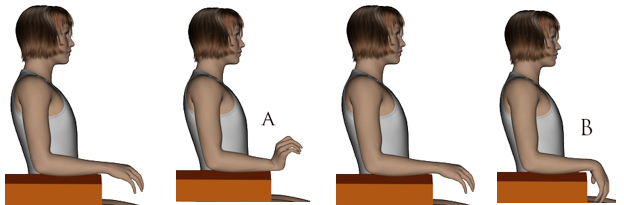
\includegraphics[width=\textwidth,keepaspectratio]{hand-extension-movements.png}
			\centering
			\caption{Exercicis de flexo-extensió de la mà.}
		\end{figure}
		\item[Mobilitat dels dits] amb la mà oberta, separar els dits en forma de ventall tot el possible i mantenir la posició 5-10 segons i tornar a la posició inicial de repòs.
		\begin{figure}[H]
			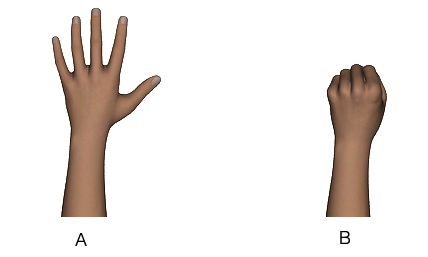
\includegraphics[width=\textwidth,keepaspectratio]{fingers-movility.jpg}
			\centering
			\caption{Exercicis d'extensió dels dits.}
		\end{figure}
		\item[Oposició del polze] dur el palpís del dit polze a la base de cada un dels altres dits començant per l'índex i acabant pel dit petit.
		\begin{figure}[H]
			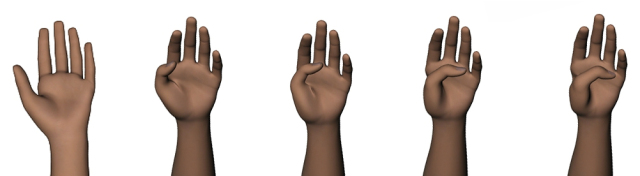
\includegraphics[width=\textwidth,keepaspectratio]{thumb-movility.jpg}
			\centering
			\caption{Exercicis d'oposició del polze.}
		\end{figure}
		\item[Mobilitat lateral del canell] amb la mà oberta, i els dits estirats, realitzar moviments amb el canell dirigint la mà primer cap a fora, mantenir 5-10 segons per a posteriorment relaxar tornant a la posició de repòs. Continuar movent la mà cap a dins, mantenir uns altres 5-10 segons i tornar a la posició inicial.
		\begin{figure}[H]
			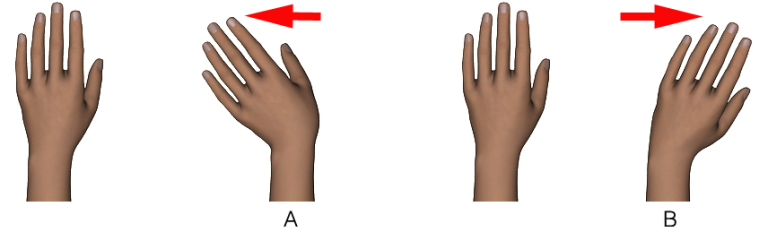
\includegraphics[width=\textwidth,keepaspectratio]{wrist-movility.jpg}
			\centering
			\caption{Exercicis de mobilitat lateral de la mà.}
		\end{figure}
	\end{description}
	\subsection{Interfícies basades en visió per a rehabilitació}
	En aquesta subsecció ens centrarem en el treball relacionat amb VBI que empren directament el moviment del cos sense la necessitat d'emprar comandaments.
	L'ús de \textit{Microsoft Kinect} (o sistemes parescuts com l'\textit{Asus Xtion}) s'han emprat per la rehabilitació de pacients amb accidents vasculars cerebrals, treball d'equilibri o que simplement necessiten recuperació física.
	
	En concret, \textit{Kinect}, presenta un grau d'utilització molt gran en aquests àmbits. \textit{Webster i Celik} \cite{webster-celik}, presenten un recull de treballs que utilitzen \textit{Kinect} per al cuidat de persones majors, per a la rehabilitació de pacients amb accidents vasculars cerebrals i exercicis basats en videojocs. Amb aplicacions tan diverses que van des de la detecció de caigudes en el cas de persones majors, fins aplicacions destinades a ajudar a que els exercicis de rehabilitació repetitius siguin més entretenguts. En el cas dels exercicis basats en videojocs, un dels treballs estudiats presenta un joc per treballar exercicis d'equilibri. En aquest joc, en el que jugador està representat per una figura humana virtual, uns contorns de figures humanes es movien cap al jugador virtual, que havia de imitar els contorns per tal de passar a través d'ells sense tocar-los.
	
	En referència a la rehabilitació de la mà, \textit{Leap motion} s'empra gràcies a la informació que ens pot donar dels dits i de la posició de la mà. Emprant aquest tecnologia, Liu et al (2015) \cite{liu-rehab} presenten un sistema on el metge pot prescriure al pacient certs moviments per imitar i aquest pot obtenir retroalimentació automàtica en forma de puntuació, d'acord amb la similitud. També es troba la utilització de videojocs per complementar la teràpia convencional (Iosa et al., 2015) \cite{losa-rehab}. Matos et al (2014) \cite{kinteract} presenten un joc per entrenar el rang d'obertura de la mà, l'usuari ha d'obrir la mà per recollir pomes i transportar-les a una cistella mantenint l'obertura de la mà. Khademi et al. (2014) juguen al Fruit Ninja emprant  la mà a rehabilitar per pacients amb accidents vascular cerebrals \cite{leap-fruit-ninja}.
	\section{Anàlisi i disseny}
	\subsection{Introducció}
	Dins aquest apartat s'analitza i descriu quin ha estat el sistema desenvolupat per tal de satisfer els objectius plantejats anteriorment.
	
	En primer lloc es presenta una descripció de l'arquitectura i les característiques del controlador \textit{Leap Motion}, que serà la interfície basada en visió que s'emprarà.
	
	Posteriorment es fa una anàlisi de requisits del sistema a desenvolupar tant des del punt de vista funcional com tecnològic, la qual cosa permet tenir una descripció detallada del sistema.
	
	Com a darrera secció es descriu el disseny de l'aplicació amb tots els seus subsistemes i els diferents jocs desenvolupats.
	\subsection{Leap Motion}
	\subsubsection{Hardware: Leap motion}
	El \textit{Leap motion} és un petit dispositiu que es connecta mitjançant USB i que és capaç de capturar els moviments de mans i dits, així com gestos o moviments de llapis (stylus) a través de dues càmeres i tres LEDs infraroigs. El dispositiu és capaç de capturar les dades de les mans fins a una distància d'uns 60 cm, tant a la part superior com als laterals del dispositiu, gràcies al gran camp de visió de les càmeres (uns 150\textdegree) \cite{leapcharacteristics}.
	\begin{figure}[H]
		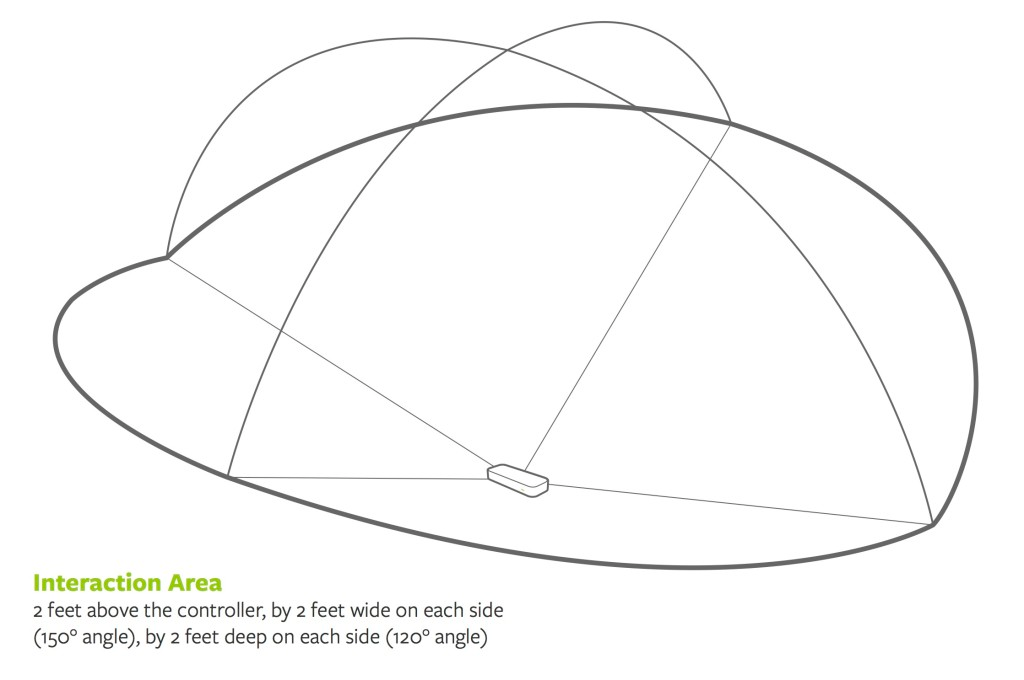
\includegraphics[width=\textwidth,keepaspectratio]{leap-motion-interaction-area.png}
		\centering
		\caption{Representació del dispositiu i el seu camp de visió \protect\cite{leapcharacteristics}.}
	\end{figure}
	Les dades capturades per aquestes càmeres són enviades per USB a l'ordinador al qual es connecta el controlador \textit{Leap}, on el software de \textit{Leap Motion}, que s'executa com un servei, s'encarrega de processar-les i deixar-les disponibles perquè puguin ser obtingudes mitjançant APIs.
	
	El servei del \textit{Leap Motion} proporciona la informació a les APIs en forma d'una sèrie de fotogrames que contenen tota la informació de seguiment capturada. Al final és competència d'aquestes APIs proporcionar a l'usuari les dades en forma d'estructures orientades a objectes, així com també proporcionar una sèrie de funcions que permeten operar amb aquestes dades.
	\subsubsection{Arquitectura del Leap Motion}
	El \textit{Leap Motion} és capaç de funcionar en múltiples sistemes operatius i les seves dades poden ser obtingudes de dues formes: mitjançant una interfície nativa o a través d'un servidor de \textit{Web socket}. D'aquesta manera, les possibilitats per als desenvolupadors són molt diverses i inclouen molts dels llenguatges de programació més utilitzats actualment \cite{leapsdkdocs}.
	
	\paragraph{Interfície nativa}
	La interfície nativa es proporciona a través d'una llibreria que connecta el servei del \textit{Leap Motion}. Aquest servei després proveeix les dades de seguiment obtingudes a les aplicacions desenvolupades. La llibreria es pot utilitzar directament en el cas d'aplicacions desenvolupades amb C++ i Objective C, o es poden utilitzar una de les APIs per Java, C\# o \textit{Python} \cite{leapsdkdocs}.
	\begin{figure}[H]
		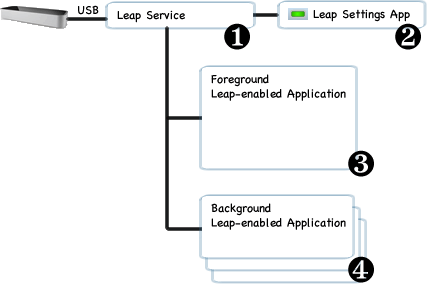
\includegraphics[width=\textwidth,keepaspectratio]{native-interface.png}
		\centering
		\caption{Esquema d'aplicacions utilitzant la interfície nativa.}
		\label{fig:native-interface}
	\end{figure}
	A continuació es descriuen les diferents parts que intervenen en la connexió del dispositiu mitjançant la interfície nativa representada a la figura \ref{fig:native-interface}.
	\begin{enumerate}
		\item El servei de \textit{Leap Motion} rep les dades del controlador a través d'una connexió USB, processa les dades rebudes i les envia a les aplicacions. Per defecte el servei només envia informació a les aplicacions en primer pla, però les aplicacions poden demanar rebre dades també en segon pla.
		\item L'aplicació de \textit{Leap Motion} és independent del servei i permet als usuaris configurar la seva instal·lació de \textit{Leap Motion}.
		\item Una aplicació en primer pla rep dades de seguiment del servei de \textit{Leap Motion}.
		\item Quan una aplicació perd el focus del sistema operatiu, el servei de \textit{Leap Motion} deixa d'enviar-li dades. Les aplicacions dissenyades per funcionar en segon pla poden demanar al servei que els proveeixi dades de seguiment fins i tot en segon pla.
	\end{enumerate}
	
	\paragraph{Interfície web socket}
	El servei de \textit{Leap Motion} executa un servidor de \textit{web socket} local en el domini local (\textit{localhost}) a través del port 6437. Aquesta interfície de web socket proveeix dades de seguiment en format JSON. Després un client \textit{JavaScript} desenvolupat per la mateixa empresa de \textit{Leap Motion}, s'encarrega de capturar aquestes dades i presentar-les com a objectes de \textit{JavaScript} estàndard.
	\begin{figure}[H]
		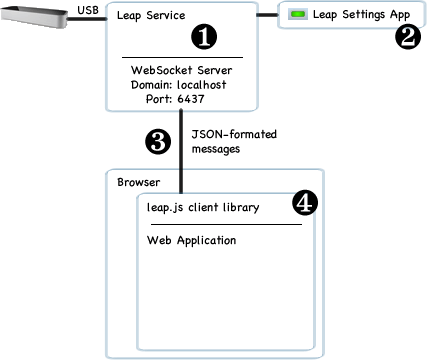
\includegraphics[width=\textwidth,keepaspectratio]{websocket-interface.png}
		\centering
		\caption{Esquema d'aplicacions utilitzant la interfície de web socket.}
		\label{fig:websocket-interface}
	\end{figure}
	Tot seguit es descriuen les diferents parts que intervenen en la connexió del dispositiu mitjançant \textit{web socket}, representat a la figura \ref{fig:websocket-interface}
	\begin{enumerate}
		\item El servei de \textit{Leap Motion} proveeix un servidor de \textit{web socket} a través de la direcció \textit{http://127.0.0.1:6437}.
		\item L'aplicació de configuració del \textit{Leap Motion} permet habilitar o deshabilitar el servidor de \textit{web socket}.
		\item El servidor envia les dades de seguiment en format JSON. Les aplicacions també poden enviar missatges de configuració al servidor.
		\item La mateixa empresa de \textit{Leap Motion} ens proveeix d'una llibreria \textit{JavaScript} que pot ser utilitzada per les aplicacions web per accedir a les dades de seguiment del \textit{Leap Motion}.
	\end{enumerate}
	Aquesta interfície està dissenyada per ser utilitzada per aplicacions web, tot i que qualsevol aplicació pot establir una connexió amb el servidor de web socket. Aquest servidor segueix l'estàndard de web socket RFC6455.
	\subsubsection{Leap Motion API}
	El sistema \textit{Leap Motion} realitza un seguiment de les mans i els dits. El dispositiu ofereix una gran precisió i una alta taxa de fotogrames per segon, i retorna valors discrets de posició i moviment.
	
	Els sensors es dirigeixen cap a l'eix Y, (cap amunt, quan el controlador es situa en la seva posició de funcionament estàndard) i com s'ha comentat anteriorment, ofereix un camp de visió d'uns 150\textdegree.
	\paragraph{Sistema de coordenades}
	El sistema \textit{Leap Motion} utilitza un sistema de coordenades cartesianes. L'origen d'aquest sistema de coordenades es situa a la part superior del dispositiu. Els eixos X i Z es situen en el pla horitzontal, amb l'eix X paral·lel a l'eix més llarg del dispositiu. L'eix Y és vertical amb valors més positius cap amunt. L'eix Z té valors positius en direcció a l'usuari i valors negatius del dispositiu en direcció contraria a l'usuari.
	\begin{figure}[H]
		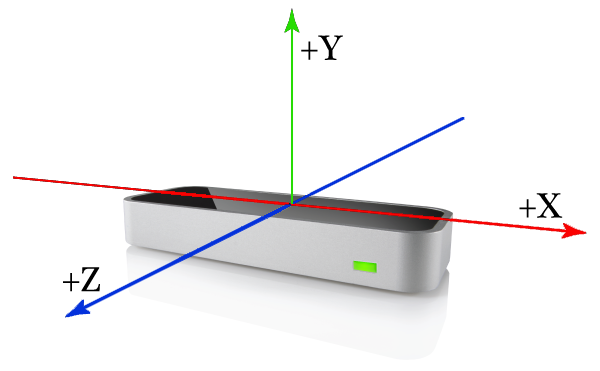
\includegraphics[width=\textwidth,keepaspectratio]{leap-coordinates.png}
		\centering
		\caption{Sistema de coordenades del \textit{Leap Motion}.}
		\label{fig:leap-coordinates}
	\end{figure}
	La API mesura les quantitats físiques en les següents unitats.\\
	
	\begin{tabular}{ l c l }
		\hline
		Distància & & mil·límetres\\ \hline
		Temps & & microsegons\\ \hline
		Velocitat & &  mil·límetres / segon\\ \hline
		Angles & & Radians\\
	\end{tabular}
	
	\vspace{5mm}
	Mentre el dispositiu fa un seguiment de les mans i dits en el seu camp de visió, proveeix actualitzacions de les dades com un conjunt de fotogrames (\textit{frames}) de dades. Cada objecte \textit{frame} conté qualsevol mà detectada, detallant les seves propietats en un únic instant de temps. L'objecte \textit{Frame} és essencialment, l'origen del model de dades retornat per la API.
	Aquesta posa a disposició dels desenvolupadors les següents classes.
	
	\paragraph{Hands}
	Les mans es representen mitjançant la classe \textit{Hand} i proveeix informació sobre la identitat, posició i altres característiques de la mà detectada. Llista també tots els dits, així com també el braç al qual està lligada la mà.
	\begin{figure}[H]
		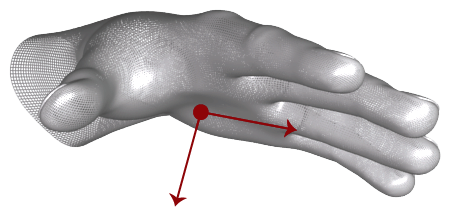
\includegraphics[width=\textwidth,keepaspectratio]{leap-hand-model.png}
		\centering
		\caption{Representació d'una mà i els vectors palmNormal i direction.}
		\label{fig:leap-hand}
	\end{figure}
	El software del \textit{Leap Motion} utilitza un model intern de la mà per tal d'oferir un seguiment predictiu, fins i tot quan parts de la mà no són visibles per els sensors. La classe \textit{Hand} ofereix una propietat \textit{Hand.confidence}, que indica en quin nivell d'exactitud encaixa en el model intern, la mà detectada.
	
	Tot i que el dispositiu és capaç de detectar més de dues mans si més d'una persona està dins el camp de visió. Es recomana limitar les mans a dues per maximitzar la qualitat de les dades de seguiment.
	\paragraph{Arms}
	\textit{Hand.arm} és un objecte que proporciona informació sobre l'orientació, longitud, amplada i punts finals d'un braç. Quan el colze està fora del camp de visió el sistema estima la posició del braç basant-se en observacions passades, així com amb les proporcions normals d'un braç humà.
	\paragraph{Fingers}
	Proporciona informació de cada dit de la mà. En cas que part d'un dit, o fins i tot tot el dit, no sigui visible, les característiques s'estimen en base a observacions recents i del model intern de la mà. Aquests dits s'identifiquen amb el seu nom en anglès (\textit{thumb}, \textit{index}, \textit{middle}, \textit{ring} i \textit{pinky}).
	\begin{figure}[H]
		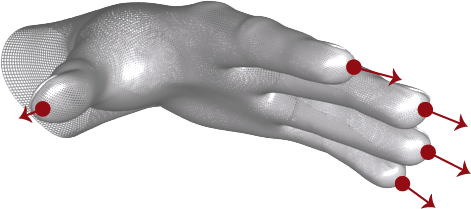
\includegraphics[width=\textwidth,keepaspectratio]{leap-fingers-model.png}
		\centering
		\caption{Representació d'una mà i els vectors de direcció dels dits.}
		\label{fig:leap-hand-fingers}
	\end{figure}
	Els objectes del tipus \textit{Finger} conté objectes de la classe \textit{Bone} que descriuen la posició i orientació de cada os del dit. Tots els dits contenen 4 ossos, ordenats de la base a la punta dels dits.
	\begin{figure}[H]
		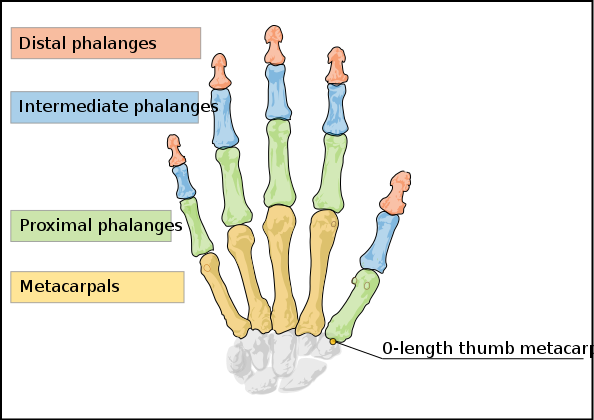
\includegraphics[width=\textwidth,keepaspectratio]{hand-bones.png}
		\centering
		\caption{Representació dels diferents ossos de la classe Hand.}
		\label{fig:hand-bones}
	\end{figure}
	Els ossos s'identifiquen de la següent manera:
	\begin{description}
		\item[Metacarpal] el \textit{metacarpal} (metacarpià) és l'os situat dins la mà, que connecta el dit al canell (excepte el polze).
		\item[Proximal Phalanx] \textit{proximal phalanx} (primera falange) és l'os de la base del dit, connectat al palmell.
		\item[Intermediate Phalanx] l'\textit{intermediate phalanx} (segona falange) és l'os intermig del dit, situat entre la punta i la base del dit.
		\item[Distal Phalanx] el \textit{distal phalanx} (tercera falange) és el darrer os del dit, situat a la punta del dit.
	\end{description}
	Per mantenir una coherència, el model del polze no reflecteix el model anatòmic real. Un polze real té un os menys que la resta de dits, en canvi el model retornat per la API conté un metacarpià de longitud 0 per tal de tenir el mateix número d'ossos que la resta de dits.
	\subsection{Requeriments}
	Tot i que l'objectiu principal del projecte és realitzar una prova de concepte per confirmar que és possible utilitzar el controlador \textit{Leap Motion} per complementar i monitorar teràpies de rehabilitació, és important establir una sèrie de requeriments tècnics i funcionals del projecte per tal de definir bé el seu abast.
	\subsubsection*{Requeriments d'usuari}
	\begin{description}
		\item [RU1] Un usuari ha de poder seleccionar un exercici a realitzar d'una llista.
		\item [RU2] Un usuari ha de poder realitzar exercicis d'extensió del canell.
		\item [RU3] Un usuari ha de poder realitzar exercicis d'abducció i adducció del canell.
		\item [RU4] Un usuari ha de poder realitzar exercicis d'abducció i adducció dels dits.
		\item [RU5] Un responsable de la rehabilitació d'un usuari ha de ser capaç de reproduir les sessions d'exercicis dels usuaris.
	\end{description}
	\subsubsection*{Requeriments funcionals dels jocs}
	\begin{description}
		\item [RF1] Els jocs han de ser el més intuïtius possibles.
		\item [RF2] Els jocs han d'engrescar als usuaris a realitzar els exercicis.
		\item [RF3] Els jocs han d'enviar les dades de seguiment dels moviments.
		\item [RF4] Cada joc ha de permetre als usuaris realitzar un sol exercici.
	\end{description}
	\subsubsection*{Requeriments no funcionals}
	\begin{description}
		\item [RNF1] Els jocs han de poder ser executats a qualsevol sistema operatiu.
		\item [RNF2] Els usuaris no han d'instal·lar cap aplicació addicional llevat dels controladors del dispositiu \textit{Leap Motion}.
	\end{description}
	\subsection{Arquitectura del sistema}
	Una vegada definits els requeriments del projecte, a continuació es presenta una descripció de l'arquitectura dissenyada per tal de satisfer aquests requeriments.
	
	Un dels objectius ha estat des del primer moment que l'accés a l'aplicació fos el més fàcil possible per part dels usuaris. Per això es va decidir que el millor era que les aplicacions s'executassin en un entorn web.
	
	Una aplicació web té l'avantatge de ser multiplataforma, és independent del sistema operatiu que tingui l'usuari el qual facilita l'accés a l'aplicació.
	
	En el nostre cas s'utilitza una arquitectura web tradicional que consta d'un servidor web que és l'encarregat de servir les aplicacions de rehabilitació als usuaris. Aquestes aplicacions contenen la major part de la lògica de l'aplicació. L'arquitectura presenta una peculiaritat, fora del que és una aplicació web tradicional, que és la utilització d'un servidor de \textit{web socket} que s'encarrega de rebre les dades del dispositiu \textit{Leap Motion} dels usuaris i guardar aquestes dades en fitxers per a que puguin ser reproduïts posteriorment pels responsables de les teràpies de rehabilitació.
	
	\begin{description}
		\item [Aplicacions web de rehabilitació] aquestes aplicacions són les encarregades de connectar-se al dispositiu \textit{Leap Motion} dels usuaris per tal que aquests puguin realitzar els exercicis.
		\item [Servidor web] un servidor web tradicional encarregat de servir les pàgines web als usuaris. També ha de ser l'encarregat de gestionar totes les dades dels usuaris per a que els responsables de la teràpia puguin fer un seguiment de les sessions de rehabilitació dels usuaris.
		\item [Servidor web socket] és un servidor que habilita una comunicació bidireccional en temps real amb els usuaris. Aquest servidor s'encarrega de guardar les dades enviades pels dispositius \textit{Leap Motion} dels usuaris per tal que aquestes puguin ser monitorades posteriorment.
	\end{description}
	\subsection{Disseny dels jocs}
	Per tal de satisfer els requeriments plantejats anteriorment, s'han dissenyat tres jocs diferents.
	
	Cada joc està dissenyat per treballar un tipus d'exercici determinat. Això implica que la complexitat del joc no pot ser molt elevada, ja que el control que pot arribar a tenir l'usuari sobre el joc, realitzant una mateixa acció repetidament és baix. A més, no s'ha d'oblidar que l'objectiu principal dels jocs no és el simple entreteniment de l'usuari, sinó que el més important és que l'usuari es senti motivat per realitzar els exercicis de rehabilitació i els realitzi de manera correcta.
	
	A més s'ha desenvolupat una aplicació de monitoratge, que podria ser utilitzada pels responsables de de la rehabilitació per dur a terme un seguiment de l'evolució dels usuaris.
	\subsubsection{Runner boy - Exercici d'extensió del canell}
	Aquest joc, està específicament dissenyat per treballar el moviment d'extensió del canell.
	És un joc de desplaçament lateral infinit on l'usuari agafa el control d'una persona o jugador, que va corrent per l'escenari del joc com es mostra a la figura \ref{fig:runnerboy-simple}.
	\begin{figure}[H]
		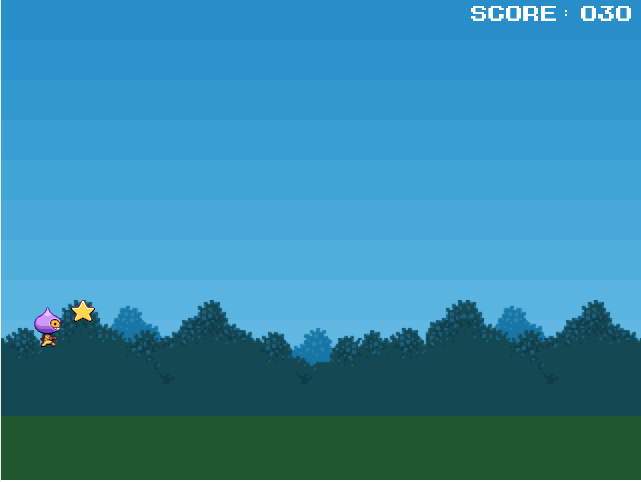
\includegraphics[width=0.8\textwidth,keepaspectratio]{runner-boy-simple.png}
		\centering
		\caption{Imatge del jugador saltant per capturar una estrella.}
		\label{fig:runnerboy-simple}
	\end{figure}
	L'objectiu és capturar unes estrelles que van apareixent en direcció contraria a l'usuari per obtenir punts. Per tal d'afegir complexitat al joc també apareixen uns obstacles que l'usuari ha d'esquivar per no perdre la partida. A més, a mesura que la puntuació de l'usuari es va incrementant, també ho fa la velocitat a la que es desplaça el joc, tant els obstacles com les estrelles de puntuació.
	
	L'usuari controla el joc per mitjà del dispositiu \textit{Leap Motion}. El primer té la capacitat de fer botar el jugador, per tal d'obtenir les estrelles que s'acosten per l'aire o d'esquivar els obstacles que apareixen per terra. El jugador realitza el moviment de salt quan l'usuari estén el canell, elevant els dits de la mà per sobre del canell tant com li sigui possible.\ref{fig:runnerboy-obstacle}.
	\begin{figure}[H]
		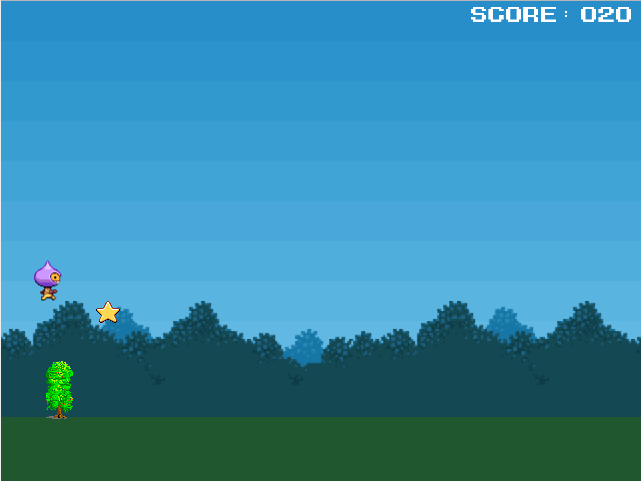
\includegraphics[width=0.8\textwidth,keepaspectratio]{runner-boy-obstacle.png}
		\centering
		\caption{Imatge del jugador esquivant un obstacle durant la partida.}
		\label{fig:runnerboy-obstacle}
	\end{figure}
	El jugador realitza el moviment de salt quan l'usuari estén el canell, elevant els dits de la mà per sobre del canell tant com li sigui possible.
	\subsubsection{Cubes road - Exercici d'abducció i adducció del canell}
	En aquest joc, els usuaris treballen els moviments d'abducció i adducció del canell de la mà. Es tracte d'un joc en 3 dimensions, en el que uns cubs es mouen a través d'una carretera en direcció a l'usuari, aquest ha d'intentar capturar-los desplaçant lateralment un altre cub.
	
	L'objectiu del joc és capturar la major quantitat de cubs possibles, incrementant així la puntuació de l'usuari. A mesura que la puntuació de l'usuari augmenta, també ho fa la velocitat a la que es desplacen els objectes cap a ell augmentant així la dificultat del joc.
	\begin{figure}[H]
		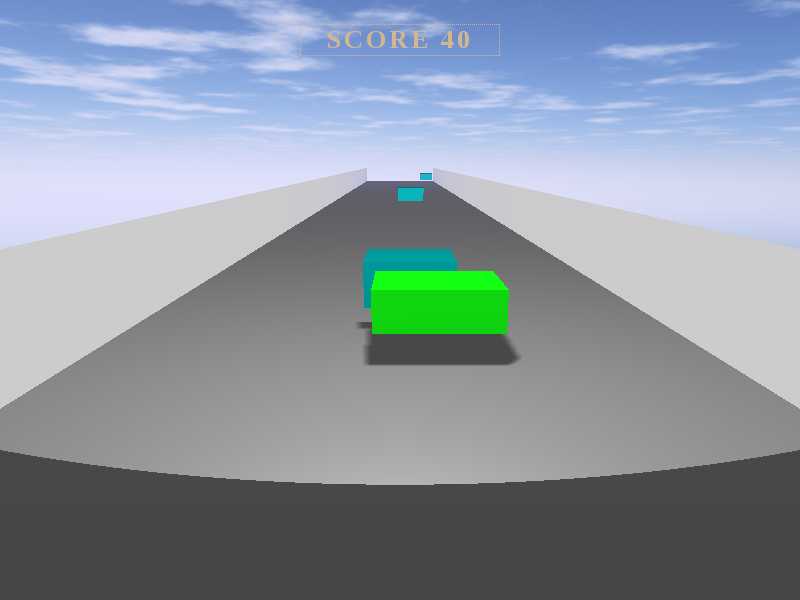
\includegraphics[width=0.8\textwidth,keepaspectratio]{cubes-road-simple.png}
		\centering
		\caption{Situació normal del joc.}
		\label{fig:cubes-road-simple}
	\end{figure}
	Amb l'objectiu d'augmentar la complexitat del joc i la motivació dels usuaris, periòdicament van apareixent uns cubs d'un color diferent que l'usuari haurà d'esquivar. En cas que l'usuari sigui incapaç d'esquivar algun d'aquests cubs que podríem denominar cubs enemics, la mida del cub que utilitza l'usuari per capturar els objectes es va reduint, d'aquesta manera com més errors comet l'usuari més difícil és per ell seguir amb la partida.
	
	La figura següent mostra l'estat del jugador després d'haver capturat per error varis cubs enemics, així com l'aspecte d'un d'aquests cubs enemics.
	\begin{figure}[H]
		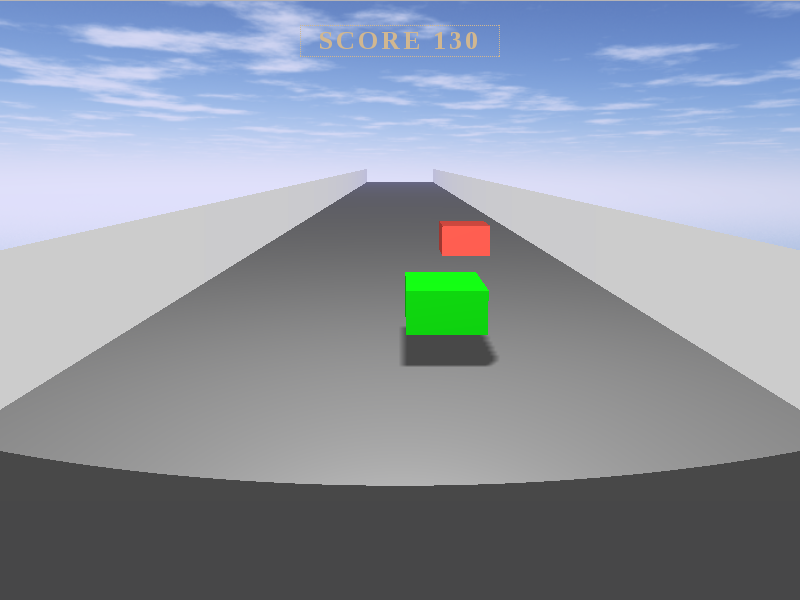
\includegraphics[width=0.8\textwidth,keepaspectratio]{cubes-road-enemy.png}
		\centering
		\caption{Imatge del jugador després d'haver col·lisionat amb varis enemics.}
		\label{fig:cubes-road-enemy}
	\end{figure}
	El moviment horitzontal del cub capturador (verd) es duu a terme mitjançant moviments d'abducció i adducció de la mà.
	\subsubsection{Catch stars - Exercici d'abducció i adducció del dits}
	Aquest darrer joc, ha estat dissenyat per treballar els exercicis d'abducció i adducció dels dits cor i anular. El moviment consisteix en separar els dits un de l'altre tant com sigui possible i tornar-los a ajuntar.
	
	Es tracta d'un joc en 2D de desplaçament vertical, on l'usuari ha de capturar unes estrelles, que van caient, per augmentar la seva puntuació. Per capturar les estrelles, els usuaris han de desplaçar horitzontalment uns cubs vermells, que hi ha a la part inferior de la pantalla, per tal de fer-los col·lisionar amb aquestes estrelles.
	\begin{figure}[H]
		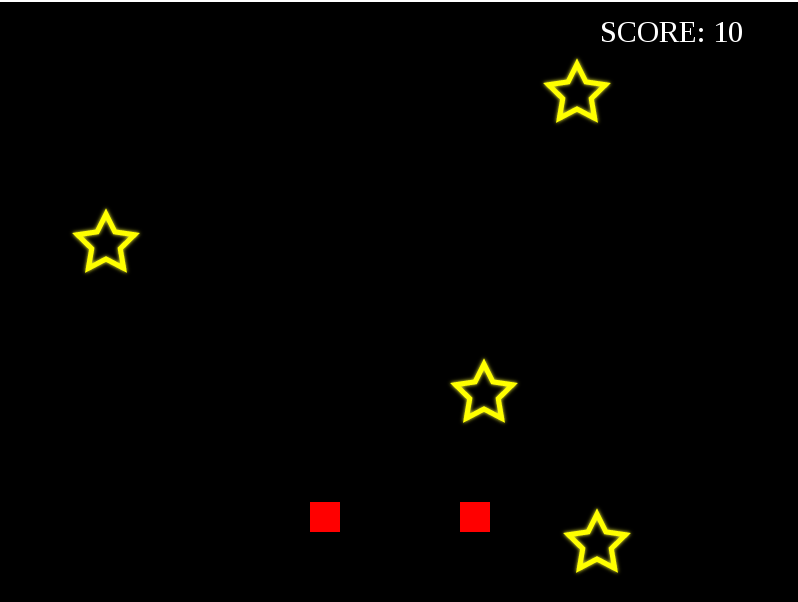
\includegraphics[width=0.8\textwidth,keepaspectratio]{catch-stars-simple.png}
		\centering
		\caption{Imatge que mostra els diferents components del joc.}
		\label{fig:catch-stars-simple}
	\end{figure}
	\subsection{Aplicació de monitoratge}
	Aquesta aplicació permet als responsables de les teràpies de rehabilitació monitorar les sessions d'exercicis que fan els seus pacients. D'aquesta manera un responsable pot avaluar la millora d'un pacient. De la mateixa manera es poden detectar errors en la realització dels exercicis.
	
	L'aplicació de monitoratge consta de 3 parts fonamentals, un \textit{plugin} del controlador \textit{Leap Motion}, un servidor de \textit{web socket} i una aplicació de reproducció dels moviments capturats pel controlador \textit{Leap} del pacient. La següent figura mostra un esquema de l'arquitectura de l'aplicació de monitoratge.
	\begin{figure}[H]
		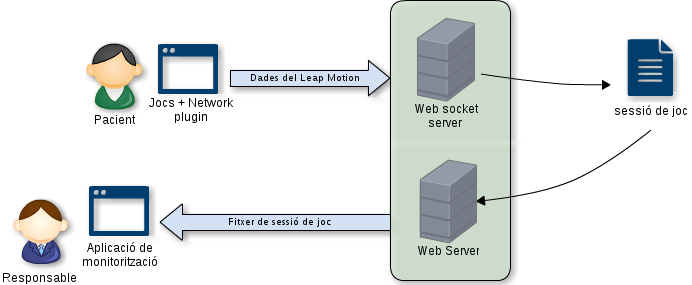
\includegraphics[width=0.8\textwidth,keepaspectratio]{esquema-monitoritzacio.png}
		\centering
		\caption{Arquitectura de l'aplicació de monitorització.}
		\label{fig:arquitectura-monitoratge}
	\end{figure}
	Així, un pacient es connecta a un dels jocs definits anteriorment, i mentre l'usuari juga, un \textit{plugin} del \textit{Leap Motion} va enviant les dades capturades a un servidor de \textit{web socket} utilitzant una estructura determinada, a la vegada, aquest servidor s'encarrega de guardar les dades rebudes a un fitxer. Després en un altre moment, un dels responsables de la teràpia d'aquest pacient, es connecta a l'aplicació de monitoratge per tal de reproduir la sessió de joc del seu pacient. En aquest cas el servidor web l'únic que fa es servir les aplicacions als usuaris i el fitxer de la sessió de joc cap a l'aplicació de monitoratge.
	\begin{description}
		\item[Network plugin] aquest és un \textit{plugin} que segueix la mateixa filosofia que els \textit{plugins} ja disponibles pel \textit{Leap Motion} \cite{leapjsplugins}. El primer que fa el \textit{plugin} és connectar-se a un servidor de web socket. Després quan el controlador \textit{Leap Motion} comença a enviar dades, aquest \textit{plugin} les captura i les envia al servidor de \textit{socket} utilitzant una estructura determinada.
		\item[Web socket] un servidor de \textit{web socket} tradicional que accepta connexions del \textit{plugin} del \textit{Leap Motion} i escolta els esdeveniments d'aquestes connexions. Quan rep una connexió nova, crea un fitxer de text i una vegada creat el fitxer de text, va escrivint les dades rebudes a través del \textit{socket} al fitxer de text en format JSON. Una vegada que el \textit{plugin} tanca la connexió amb el servidor, aquest darrer rep un esdeveniment de desconnexió i deixa el fitxer disponible per ser reproduït per l'aplicació de monitoratge.
		\item[Visor de monitoratge] és una aplicació web que es connecta al controlador \textit{Leap Motion}, i utilitza les dades del fitxer, creat pel servidor de socket, per reproduir els moviments de la mà que ha realitzat l'usuari del joc.
		
		Com si es tractàs d'un fitxer de vídeo, aquesta aplicació permet pausar la reproducció dels moviments, així com moure's endavant i enrere. Per tal de facilitar la revisió dels moviments, els usuaris d'aquesta aplicació també tenen la capacitat de rotar la mà que es veu a la reproducció i modificar el zoom de la imatge.
	\end{description}
	La següent imatge mostra com veuen els responsables de les teràpies, la reproducció dels exercicis realitzats pels seus pacients.
	\begin{figure}[H]
		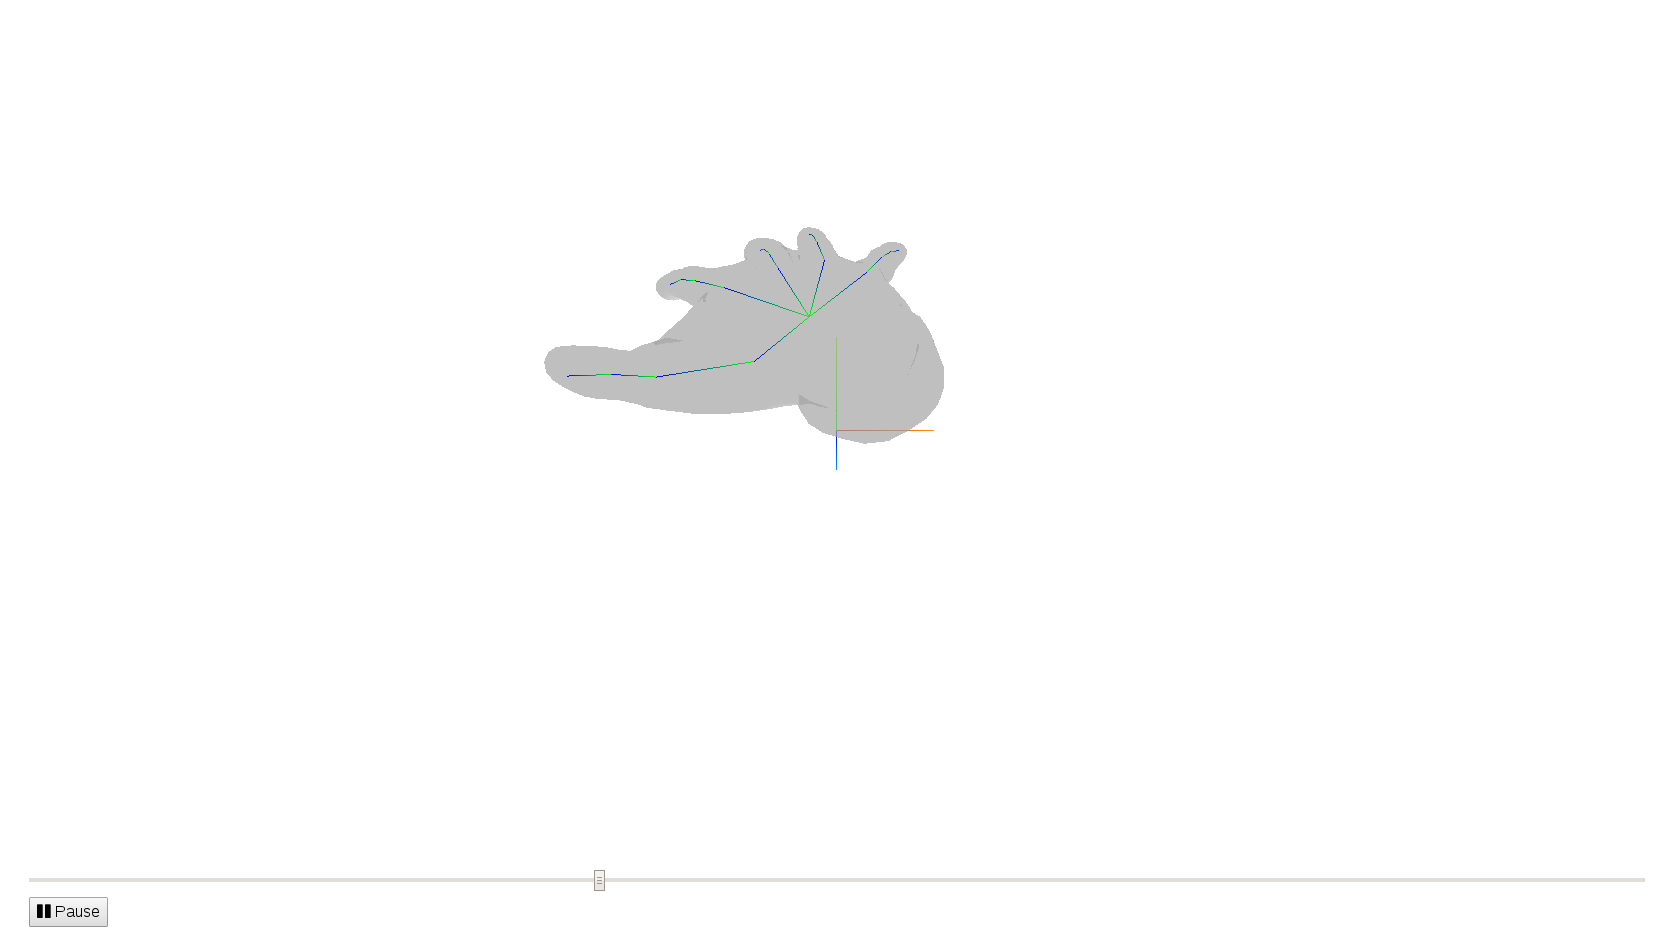
\includegraphics[width=0.8\textwidth,keepaspectratio]{playback-simple.png}
		\centering
		\caption{Visor de l'aplicació de monitoratge.}
		\label{fig:playback-simple}
	\end{figure}
	\section{Implementació}
	En aquest apartat es descriuen els detalls d'implementació de les diferents aplicacions i sistemes desenvolupats.
	
	Primer, es presenten les tecnologies utilitzades per desenvolupar les aplicacions i les raons per les quals s'han triat aquestes tecnologies, i després es detallen els aspectes més interessants de la implementació de les diferents aplicacions.
	
	\subsection{Tecnologies utilitzades}
	Durant la implementació de les aplicacions i sistemes dissenyats s'han utilitzat les següents tecnologies i llenguatges de programació.
	\begin{description}
		\item[HTML, CSS] són la base de l'estructura i el disseny de qualsevol aplicació web.
		\item[JavaScript] és el llenguatge de programació utilitzat pels navegadors web.
		\item[Node.js] és un entorn multiplataforma que permet executar codi JavaScript a la banda del servidor. Presenta una arquitectura basada en esdeveniments i que permet l'execució d'operacions d'entrada i sortida de manera asíncrona. Aquestes prestacions tenen l'objectiu de maximitzar la productivitat d'aplicacions amb múltiples operacions d'entrada i sortida, així com facilitar la implementació d'aplicacions web de temps real \cite{nodejs}.\\
		Aquestes característiques fan que aquesta tecnologia sigui una de les més adequades per a la implementació del servidor de web socket, ja que aquesta rebrà moltes peticions i haurà de realitzar operacions d'escriptura per a cada petició.
	\end{description}
	Per altra banda s'han utilitzat diverses llibreries que han ajudat a implementar les diferents aplicacions, en especial a l'hora la programació dels videojocs.\\
	\begin{description}
		\item[Express.js] és un \textit{framework} per al desenvolupament de servidors web amb \textit{Node.js}.
		\item[Socket.io] és una llibreria per a \textit{JavaScript} per a la implementació d'aplicacions web de temps real. Consta de dues parts, una llibreria client que s'executa al navegador i una llibreria per al servidor (\textit{Node.js}). Proporciona un gran ventall de prestacions al voltant de \textit{web socket}.
		\item[Phaser.io] és una llibreria per al desenvolupament de videojocs \textit{HTML5} en 2d.
		\item[Three.js] és una llibreria \textit{JavaScript} que permet la creació de gràfics en 3 dimensions per a navegadors web.
		\item[Physijs] és un \textit{plugin} per a \textit{Three.js} que facilita la gestió de càlculs físics. Afegeix prestacions com gravetat, gestió de col·lisions, rebots, etc, a una escena de \textit{Three.js}.
		\item[TweenMax] és una llibreria per a la gestió d'animacions complexes en \textit{Javascript}.
		\item[Leapjs Plugin] és un \textit{plugin} per al \textit{software} de \textit{Leap Motion} per a \textit{JavaScript} que permet la reproducció dels fotogrames capturats pel controlador \textit{Leap Motion}. Utilitzat en la implementació de l'aplicació de monitoratge.
		\item[Webpack] és un agregador de mòduls per a \textit{JavaScript}. La seva funció és recopilar els mòduls que utilitza una aplicació i generar un sol fitxer estàtic que representa aquells mòduls. Això ens permet mantenir un enfocament modular a l'hora de desenvolupar aplicacions web.
	\end{description}
	\begin{figure}[H]
		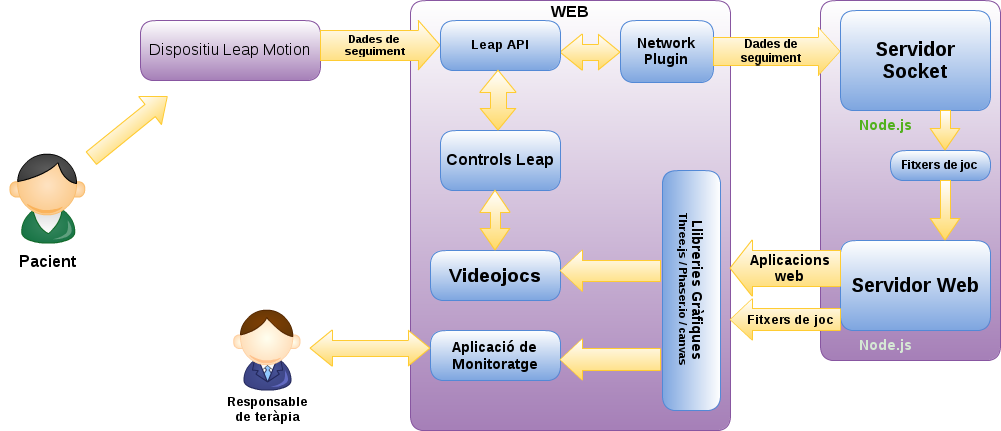
\includegraphics[width=0.8\textwidth,keepaspectratio]{technologies.png}
		\centering
		\caption{Relació entre les diferents tecnologies utilitzades.}
		\label{fig:technolgies}
	\end{figure}
	\subsection{Detalls d'implementació}
	Per al desenvolupament del projecte i la consecució dels objectius prevists, s'han implementat els següents sistemes i aplicacions.
	\begin{description}
		\item[Servidor web] encarregat de servir les aplicacions web i els fitxers estàtics necessaris per al funcionament d'aquestes.
		\item[Servidor web socket] Utilitzat per guardar les dades de seguiment dels dispositius \textit{Leap Motion} dels usuaris, per tal que puguin ser reproduïts posteriorment quan es desitgi.
		\item[Runner boy] videojoc \textit{HTML5} desenvolupat utilitzant la llibreria \textit{Phaser.io}. Està dedicat a exercitar el moviment de flexió del canell.
		\item[Cubes Road] videojoc \textit{HTML5} en 3D desenvolupat utilitzant la llibreria \textit{Three.js}. Té com a objectiu exercitar els moviments d'abducció i adducció del canell.
		\item[Catch Stars] videojoc \textit{HTML5} desenvolupat únicament amb l'element \textit{HTML5} \textit{canvas}. L'objectiu principal d'aquest joc és exercitar els moviments d'abducció i adducció dels dits cor i anular. D'altra banda un altre objectiu d'implementar el joc utilitzant només la API dels elements canvas, ha estat comparar com és la creació d'un videojoc utilizant APIs bàsiques com les de \textit{canvas}, en vers a la utilització de llibreries com \textit{Phaser.io} i \textit{Three.js} que faciliten molts processos.
		\item[LeapJS Network plugin] \textit{plugin} propi desenvolupat seguint la filosofia dels \textit{plugins} ja disponibles per \textit{Leapjs}. La seva funció és enviar les dades de seguiment del controlador \textit{Leap Motion}, a un servidor de \textit{web socket}.
		\item[Aplicació de monitoratge] una aplicació web que utilitza el \textit{plugin} \textit{leapjs-playback} per reproduir les dades de seguiment del \textit{Leap Motion}. Per tal de reproduir els moviments, utilitza el fitxer guardat pel servidor de \textit{web socket}.
	\end{description}
	A continuació es descriuen de manera detallada els aspectes més interessants de la implementació d'aquests sistemes i aplicacions.
	\subsubsection{Servidor web}
	És tracta d'un servidor web bàsic, implementa les funcionalitats necessàries per donar servei als diferents videojocs desenvolupats.
	
	S'ha desenvolupat utilitzant el \textit{framework} \textit{Express.js} ja que aquest simplifica moltes de les configuracions que necessita una servidor web, és pot implementar un servidor web senzill amb un parell de línies de codi.
	\begin{figure}[H]
		\begin{lstlisting}[gobble=12, tabsize=4]
			const express = require('express');
			const app = express();
			
			const PORT = 3000;
			app.get('/greeting', (req, res) => {
			  res.send('Hello World!');
			})
			
			app.use(
				express.static(path.resolve(__dirname, 'games')));
			
			app.listen(PORT, () => {
			  console.log(`App listening on port ${PORT}!`);
			});
		\end{lstlisting}
		\caption{Codi bàsic d'un servidor Express.js.}
		\label{fig:express-basic}
	\end{figure}
	\subsubsection{Servidor socket}
	Aquest servidor, desenvolupat mitjançant la llibreria \textit{Socket.io}, s'encarrega de rebre les connexions del \textit{plugin} de \textit{Leap Motion} i generar els fitxers de les sessions de joc.
	
	El seu paper més important és generar el fitxer de les sessions de joc utilitzant l'estructura adecuada, que després podrà ser reproduïda utilitzant el \textit{plugin} de reproducció \textit{leapjs-playback}. A continuació es mostra quina és l'estructura de dades que ha de guardar el servidor de \textit{web socket} en el fitxer.
	\begin{figure}[H]
		\begin{lstlisting}[gobble=12, tabsize=4]
			{
			  metadata: {
			    formatVersion: 2,
			    generatedBy: 'Socket.io saver',
			    frames: 0,
			    protocolVersion: 6,
			    frameRate: '1.1e+2',
			    modified: new Date()
			  },
			  frames: [packingStructure]
			}
		\end{lstlisting}
		\caption{Estructura del fitxer de sessió de joc.}
		\label{fig:recording-structure}
	\end{figure}
	Les meta dades vénen determinades pel \textit{plugin} de reproducció y la majoria són constants o són regenerades a l'hora de reproducció del \textit{plugin}, com és el cas del \textit{frameRate} (ràtio de fotogrames).
	
	Les dades de seguiment del \textit{Leap} es guarden en forma de \textit{Array} de fotogrames a la propietat \textit{frames}, amb l'única peculiaritat que el primer element de la \textit{Array} descriu l'estructura amb què es guarda cada fotograma. Aquest estructura amb què es guarda cada fotograma serà descrita a l'apartat de \textit{Network Plugin}, ja que és el \textit{plugin} desenvolupat el que s'encarrega de generar les dades amb l'estructura adequada i enviar-les.
	
	El Servidor utilitza el que \textit{Socket.io} defineix com a \textit{namespace} per tal d'atendre les connexions de cada un dels jocs. Un “namespace” es pot entendre com una sala en la qual els \textit{sockets} es poden comunicar entre si, d'aquesta manera un servidor pot enviar missatges a tots els \textit{sockets} connectats a una sola sala i només als d'aquella sala.
	Es defineix una sala per a cada videojoc, d'aquesta manera:
	\begin{figure}[H]
		\begin{lstlisting}[gobble=12, tabsize=4]
			io.of('/catch-stars')
			  .on('connection', leapRecorder);
			io.of('/runner-boy')
			  .on('connection', leapRecorder);
			io.of('cubes-road')
			  .on('connection', leapRecorder);
		\end{lstlisting}
		\caption{Sales del servidor de socket}
		\label{fig:socket-namespaces}
	\end{figure}
	Com es pot veure totes les connexions a les diferents sales, són manegades per la mateixa funció \textit{leaprecorder}. Tot i que pot parèixer innecessari crear una sala per a cada videojoc, d'aquesta manera és més fàcil generar fitxers amb noms diferents per a cada videojoc, a més el codi queda més estructurat de cara al futur.
	La funció \textit{leapRecorder} rep com a paràmetre un objecte \textit{Socket} i serà a través d'aquest que es rebran els esdeveniments enviats pel \textit{plugin}.
	\begin{figure}[H]
		\begin{lstlisting}[gobble=12, tabsize=4]
			function leapRecorder(socket){
			  let fileName = socket.id.substring(socket.nsp.name.length + 1);
			  fileName = socket.nsp.name.substring(1) + '-' + fileName + '.json';
			  const ws = fs.createWriteStream(fileName);
			  const fileData = {
			    metadata: {
			      formatVersion: 2,
			      generatedBy: 'Socket.io saver',
			      frames: 0,
			      protocolVersion: 6,
			      frameRate: '1.1e+2',
			      modified: new Date()
			    },
			    frames: [packingStructure]
			  }
			  const str = JSON.stringify(fileData);
			  ws.write(str.substring(0, str.length - 2));
			
			  socket.on('disconnect', () => {
			    ws.write(']}');
			    ws.close();
			  });
			
			  socket.on('frameBuffer', data => {
			    let buffer = JSON.stringify(data[0]);
			    for (let i = 1; i < data.length; i++) {
			      buffer = buffer + ',' + JSON.stringify(data[i]);
			    }
			    ws.write(',' + buffer);
			  });
			}
		\end{lstlisting}
		\caption{Funció principal del servidor de socket}
		\label{fig:leap-recorder}
	\end{figure}
	Val la pena descriure breument el funcionament d'aquesta funció.
	Quan un client es connecta al servidor, es crea un fitxer amb l'estructura descrita anteriorment. El fitxer es guarda en format JSON (\textit{JavaScript Object Notation}, en anglès). En concret, del text resultant de convertir l'objecte a JSON, es guarda tot llevat dels dos darrers caràcters.
	\begin{lstlisting}[gobble=8, tabsize=4]
		ws.write(str.substring(0, str.length - 2));
	\end{lstlisting}
	Això serà el que permetrà anar afegint les dades rebudes periòdicament dins de l'array \textit{frames}, sense haver de regenerar cada vegada l'objecte complet.
	Així, quan el \textit{plugin} envia un missatge de dades del \textit{Leap Motion}, aquestes són afegides directament al final del fitxer en format JSON.
	\begin{figure}[H]
		\begin{lstlisting}[gobble=12, tabsize=4]
			socket.on('frameBuffer', data => {
			  let buffer = JSON.stringify(data[0]);
			  for (let i = 1; i < data.length; i++) {
			    buffer = buffer + ',' + JSON.stringify(data[i]);
			  }
			  ws.write(',' + buffer);
			});
		\end{lstlisting}
		\caption{funció que atén les dades de seguiment}
		\label{fig:socket-frame-data}
	\end{figure}
	Com es pot veure, dins del missatge de dades del \textit{plugin}, no arriba només un fotograma capturat pel \textit{Leap Motion}, sinó que arriben múltiples fotogrames. Això s'ha fet així per tal d'optimitzar la utilització de xarxa del \textit{plugin}, ja que el ràtio de fotogrames per segon produït pel controlador \textit{Leap Motion}, pot ser molt gran.
	
	Finalment, una vegada l'usuari tanca el joc, el servidor detecta la desconnexió de l'usuari i tanca el fitxer. Per tal que el fitxer contingui un JSON ben format, s'han d'afegir els dos caràcters que s'han omès a l'inici de la connexió.
	\begin{figure}[H]
		\begin{lstlisting}[gobble=12, tabsize=4]
			socket.on('disconnect', () => {
			  ws.write(']}');
			  ws.close();
			});
		\end{lstlisting}
		\caption{Event de desconnexió}
		\label{fig:socket-disconnect}
	\end{figure}
	Una vegada tancat el fitxer, aquest ja està disponible per ser reproduït per l'aplicació de monitoratge.
	\subsubsection{Runner Boy}
	Per a la implementació d'aquest joc s'ha fet servir el \textit{framework} \textit{Phaser.io}. Aquest \textit{framework}, basa l'execució dels jocs en vàries funcions principals, que podem anomenar funcions d'estat. Un objecte de la classe \textit{Phaser.Game}, pot tenir diversos estats i cada estat executa totes aquestes funcions en cas d'estar definides.
	\begin{description}
		\item[init] és la primera funció a ser cridada. S'utilitza per inicialitzar les variables inicials del joc. En el nostre cas s'utilitza per definir les variables de la mida del joc, velocitat dels objectes, gravetat, així com moltes variables auxiliars que necessitarà el joc posteriorment.
		\item[preload]: aquesta funció és cridada una vegada al principi de l'execució del joc, després de la funció \textit{init}. Aquí carregam les imatges que utilitzarà el nostre joc, per a que el \textit{framework} sigui capaç d'introduir-les a l'escena del joc més ràpidament.
		\item[create] es crida just després que la funció \textit{preload} s'hagi completat. Aquí s'afegeixen els objectes principals del joc, el fons, el terra, el jugador, etc. També és el moment en què s'inicialitzen els intervals d'inserció d'obstacles i estrelles que aniran apareixent periòdicament.
		\item[update] aquest és el bucle principal del joc. S'executarà periòdicament i és on s'han d'introduir les operacions principals d'actualització del joc, per exemple, actualitzacions de posicions d'objectes en base als algoritmes del joc. En el nostre cas com que gran part de les accions del joc estan basades en esdeveniments, ens ha quedat una funció molt senzilla, que només gestiona el moviment horitzontal del jugador.
		\item[render] la majoria d'objectes es renderitzen automàticament quan utilitzam el \textit{framework Phaser.io}, i per tant, en cas de no necessitar cap efecte de postprocessament, no fa falta s'implementi aquesta funció. En el nostre cas no ens ha calgut implementar-la.
	\end{description}
	Pot ser, la part més interessant de la implementació és la de control mitjançant el controlador \textit{Leap Motion}.
	
	Com s'ha descrit anteriorment, l'usuari té la capacitat de fer saltar el jugador realitzant moviments d'extensió del canell. Aquest és un gest que no és detectat automàticament pel servei del \textit{Leap Motion}.
	
	Per tal de detectar el gest d'extensió del canell i actuar en conseqüència sobre el joc, s'ha implementat una funció de detecció d'aquest gest.
	Un gest es pot definir com un moviment que realitza l'usuari amb la mà, i que consta d'un estat inicial que indica l'inici del gest, una sèrie de moviments de transició, i un estat final que indica la finalització del gest.
	
	En el nostre cas, l'usuari es posiciona amb la mà i el braç paral·lels al pla horitzontal, estant la mà sobre el controlador \textit{Leap Motion}. El gest comença quan l'usuari eleva els dits de la mà per damunt el braç.
	\clearpage
	\begin{wrapfigure}{l}{0.3\textwidth}
		\centering
		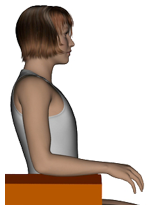
\includegraphics[width=0.3\textwidth]{hand-extension-init.png}
		\caption{Inici del gest.}
		\label{fig:hand-up-init}
	\end{wrapfigure}
	
	Per detectar aquest moviment es calcula el producte escalar entre el vector direccional del braç i el vector normal del palmell de la mà. Per calcular aquest producte s'utilitzen les components Y i Z dels vectors en tres dimensions que obtenim de la API del \textit{Leap Motion}.
	En la posició inicial on la mà i el braç tenen la mateixa direcció (en components y, z), el vector normal del palmell i el vector direccional del braç formen un angle de 90\textdegree, i per tant, el producte escalar és 0.
	
	En la realitat l'usuari no manté una posició tan estable i per tant el producte escalar no arriba a tenir un valor exacte a 0. Per això definim un valor llindar a partir del qual podem determinar amb seguretat que l'usuari ha començat a realitzar el moviment d'extensió del canell.
	
	\begin{wrapfigure}{r}{0.3\textwidth}
		\centering
		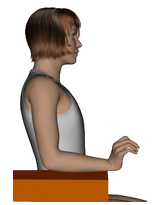
\includegraphics[width=0.3\textwidth]{hand-extension-end.png}
		\caption{Fi del gest.}
		\label{fig:hand-up-end}
	\end{wrapfigure}
	
	A partir d'aquí consideram el gest com a iniciat. Mentre l'usuari mantingui el moviment, el producte escalar seguirà augmentant i per tant podem considerar que l'usuari segueix realitzant el gest.
	
	Quan el producte vectorial deixa d'augmentar consideram que l'usuari ha arribat al màxim del moviment d'extensió i per tant podem donar el gest com a acabat.
	\clearpage
	\subsubsection{Cubes Road}
	Per implementar aquest joc s'ha utilitzat la llibreria \textit{Three.js} que permet la manipulació d'objectes 3d en navegadors web.
	
	Quan s'utilitza la llibreria \textit{Three.js} s'han de tenir en compte tres elements bàsics. Una escena, una càmera i un \textit{renderer}.
	\begin{description}
		\item[Scene] l'escena és l'objecte que utilitza \textit{Three.js} per mostrar els objectes. Una vegada creat qualsevol objecte, si volem que es mostri per pantalla, s'ha d'afegir a aquesta escena.
		\item[Camera] és l'objecte a través del qual veiem l'escena en 3 dimensions, \textit{Three.js} disposa de vàries càmeres diferents, l'estudi de les quals estaria fora de l'abast d'aquest projecte.
		\item[Renderer] l'objecte \textit{renderer} és el que utilitza \textit{Three.js} per pintar els elements per pantalla. S'ha utilitzat \textit{WebGL} per aquest propòsit, Three.js disposa d'altres “renderers” que generalment s'utilitzen en navegadors que no disposen de la tecnologia \textit{WebGL}.
	\end{description}
	La implementació es basa en 4 classes principals per gestionar el joc. La classe principal, \textit{Game}, és la classe que representa el joc i conté la major part de les funcions. La classe \textit{Cube}, és la classe que representa els cubes que ha de capturar l'usuari, a més, aquesta serveix de base per les altres dues classes principals, \textit{EnemyCube} que representa els cubs enemics que l'usuari ha d'esquivar, i \textit{Picker} que representa el jugador dintre del joc.
	A diferència del joc anterior, on la llibreria gestionava el bucle principal del joc, en aquest cas, s'ha hagut de gestionar manualment.
	
	La següent figura mostra el bucle principal del joc:
	\begin{figure}[H]
		\begin{lstlisting}[gobble=12, tabsize=4]
			animate(tFrame) {
				if (this.state === 'Playing') {
					requestAnimationFrame(this.animate.bind(this));
				}
				const pickerXPos = getPosition(
					(-roadWidth / 2) + 75, (roadWidth / 2) - 75);
				if (pickerXPos) {
					this.picker.position.x = pickerXPos;
					this.picker.needsUpdate();
				}
				if (tFrame - this.tCube > this.cubesInterval){
					if (tFrame - this.tEnemy > this.enemiesInterval) {
						this.tEnemy = tFrame;
						this.tCube = tFrame;
						this.addEnemy();
					}else {
						this.tCube = tFrame;
						this.addCube();
					}
				}
				this.handleMisses();
				this.scene.simulate();
				this.renderer.render(this.scene, this.camera);
			}
		\end{lstlisting}
		\caption{Bucle principal del joc.}
		\label{fig:cubes-road-animate}
	\end{figure}
	El bucle està controlat per la funció \textit{requestAnimationFrame} \cite{request-animation-frame}, aquesta funció avisa al navegador de que es vol realitzar una animació i fa que aquest cridi a una funció just abans del pròxim repintat de pantalla.
	
	Com es pot veure és un bucle molt senzill. A continuació es descriu breument.
	
	El primer que es controla és l'estat del joc, si el joc està en estat \textit{Playing} el bucle reserva la pròxima iteració amb la funció \textit{requestAnimationFrame}. L'estat del joc pot canviar quan el jugador perd la partida.
	
	Després es crida a la funció \textit{getPosition}, aquesta funció rep com a paràmetres un valor mínim i un màxim, la funció retorna un valor que representa la posició de la mà entre aquests dos valors. Més endavant es presenten els detalls d'implementació de la funció.
	
	A continuació, si la funció \textit{getPosition} ha retornat un valor, s'actualitza la posició a l'eix X del jugador. Recordem que el jugador només es pot moure en l'eix X per mirar de capturar els cubs. Podria ser que la funció no retornàs cap valor, perquè el controlador \textit{Leap Motion} no està connectat, i per tant no és capaç d'obtenir els valors de la mà de l'usuari.
	
	El pas següent és comprovar si cal afegir un nou cub a l'escena, aquesta comprovació consisteix en calcular el temps que ha passat des del darrer cop que es va afegir un cub al joc, si fa més temps que un determinat interval, s'afegeix un cub, sinó no. Aquest interval s'anirà fent més petit a mesura que la puntuació del jugador augmenti i per tant apareixeran cubs més sovint. Per explicar com es calcula el temps que ha passat des de la darrera vegada que es va afegir un cub, cal mencionar que la funció \textit{requestAnimationFrame}, crida a la funció que se li passa com paràmetre afegint un paràmetre addicional. Aquest paràmetre és una referència del temps que ha passat des del temps en que la navegació a la pàgina web actual va començar amb una precisió de cinc microsegons \cite{request-animation-frame}. Per si sol, aquest paràmetre no té gaire valor, però donada la precisió que ofereix pot ser utilitzat per guardar temps de referència dins el joc. Així cada vegada que s'afegeix un cub, es guarda el temps en el qual s'ha afegit utilitzant aquest valor.
	
	En el cas que s'hagi d'afegir un cub, el joc després determina quin tipus de cub s'ha d'afegir, un cub per a que el jugador obtingui més puntuació, o un cub enemic. Aquesta comprovació és fa seguint la mateixa filosofia que l'anterior, si ha passat més d'un determinat temps des de la darrera vegada que es va afegir un cub enemic, s'afegeix un cub enemic, sinó s'afegeix un cub bo, o cub de premi. Aquest interval de cubs enemics sempre serà més gran que el de cubs bons, de tal manera que sempre apareguin més cubs bons que cubs enemics.
	
	La funció \textit{handleMisses} gestiona els cubs que l'usuari no ha capturat, bé perquè aquest cub era un cub enemic i per tant l'usuari l'ha ignorat deliberadament, o bé perquè ha estat incapaç de capturar-lo. Es considera que l'usuari ha estat incapaç de capturar el cub quan la posició respecte a l'eix Z del cub és major que la posició respecte a l'eix Z de la càmera. Ja que la càmera enfoca en direcció al jugador en aquest moment el cub ja no és visible a l'escena.
	
	Si el cub és un cub enemic aquest simplement s'elimina de l'escena. En canvi si el cub és un cub de premi, el jugador l'hauria d'haver capturat i per tant es considera que el jugador ha fallat un cub, si el jugador falla 5 o més cubs perd la partida.
	
	Per acabar es criden dues funcions que no són d'implementació pròpia. Com hem pogut comprovar, el bucle no gestiona el moviment dels cubs, llevat del cub que representa el jugador, el moviment d'aquests es gestionat per la llibreria \textit{Physi.js}. Aquesta llibreria també és l'encarregada de detectar les col·lisions entre objectes de l'escena i avisar-nos mitjançant esdeveniments. El mètode \textit{simulate} de l'objecte \textit{scene} s'encarrega de demanar a la llibreria que realitzi els càlculs necessaris per determinar les noves posicions de tots els cubs de l'escena. En darrera instància, el mètode \textit{render} de l'objecte \textit{renderer} notifica a \textit{Three.js} que ha de repintar l'escena.
	
	Com s'ha mencionat en aquest apartat, la llibreria \textit{Physi.js} s'encarrega de detectar les col·lisions entre objectes per nosaltres. No obstant, no n'hi ha prou amb detectar que dos objectes han col·lisionat, sinó que s'ha d'actuar en conseqüència, i per això la llibreria permet atendre les col·lisions mitjançant esdeveniments de la mateixa manera que es fa amb els esdeveniments clàssics de JavaScript \cite{js-event}.
	
	D'aquesta manera, l'objecte joc dóna d'alta el que es coneix com a funció \textit{handler} o \textit{callback}, que és una funció que atén un esdeveniment o que és cridada per retornar la resposta a una funció, per atendre els esdeveniments de col·lisió que origina l'objecte \textit{Picker}.
	\begin{figure}[H]
		\begin{lstlisting}[gobble=12, tabsize=4]
			initPicker() {
				this.picker = new Picker(this.scene);
				this.picker.position.y = CUBES_HEIGHT;
				this.picker.position.z = PICKER_Z_POSITION;
				this.picker.addToScene();
				this.picker.addEventListener('collision', this.onCubePicked.bind(this));
			}
		\end{lstlisting}
		\caption{Inicialització de l'objecte \textit{picker}}
		\label{fig:picker-init}
	\end{figure}
	Així, cada vegada que l'objecte \textit{picker} col·lisiona amb un altre objecte dins l'escena, la funció \textit{onCubePicked} és cridada.
	\begin{figure}[H]
		\begin{lstlisting}[gobble=12, tabsize=4]
			onCubePicked(cubeMesh, relVelocity, relRotation, contactNormal){
				this.particlesHolder.spawnParticles(
				cubeMesh.position.clone(), 10, cubeMesh.material.color, .8);
				this.scene.remove(cubeMesh);
				if (this.cubesMap.get(cubeMesh) instanceof EnemyCube) {
					this.picker.shrink();
				}else {
					this.score += 10;
					this.scoreText.innerHTML = `score ${this.score}`;
					this.level = Math.floor(this.score / 50);
					if (this.score % 50 === 0) {
						this.cubesInterval = Math.max(
						this.cubesInterval - this.cubesIntervalStep, this.maxCubesInterval);
						this.velocity = Math.min(
						this.velocity + this.velocityStep, this.maxVelocity);
					}
					if (this.score % 100 === 0) {
						this.shrinkCubes();
					}
				}
				this.cubesMap.delete(cubeMesh);
			}
		\end{lstlisting}
		\caption{Funció que atén les col·lisions dels cubs.}
		\label{fig:oncubepicked}
	\end{figure}
	La funció rep varis paràmetres que donen informació sobre la col·lisió entre els objectes, l'únic que s'utilitza és el primer, que és una referència a l'objecte amb el qual ha col·lisionat el jugador. Cal recordar, que aquesta funció és un mètode de la classe principal Game i per tant, l'objecte \textit{this} fa referència a l'objecte de la classe Game.
	El primer que es fa quan es detecta una col·lisió, és generar un efecte visual que crea múltiples partícules en el lloc de la col·lisió i genera un efecte similar a una explosió, d'això se n'encarrega l'objecte \textit{particlesHolder}. No s'entrarà en més detalls per no tractar-se d'una funcionalitat del joc, sinó d'un simple efecte visual per remarcar que el jugador ha capturat un cub.
	
	Acte seguit, s'elimina el cub amb el qual ha col·lisionat l'usuari, ja que aquest cub ha estat capturat.
	
	A partir d'aquí tenim dues opcions, que el cub sigui un cub enemic, o un cub bo o de premi.
	
	Si el cub era un cub enemic: el que es fa és fer tornar l'objecte \textit{picker} una mica més petit, per tal que a l'usuari li sigui més difícil capturar els pròxims cubs.
	
	En cas que sigui un cub de premi, s'augmenta la puntuació de l'usuari en 10 punts. Llavors, es prenen una sèrie de mesures per augmentar la dificultat de la partida. Cada 50 punts l'interval entre els cubs es redueix i augmenta la velocitat a la que es mouen els cubs. A més cada 100 punts els cubs disminueixen la seva mida.
	El darrer pas és eliminar la referència al cub capturat del mapa que el joc utilitza per tenir una referència a tots els cubs que hi ha a l'escena.
	
	D'aquesta manera, el joc continua fins que l'usuari perd la partida o decideix deixar de jugar.
	
	\subsubsection{Catch Stars}
	Aquest joc, s'ha implementat sense utilitzar cap llibreria externa per poder experimentar i comparar com seria la creació d'un joc utilitzant només APIs de baix nivell, ja disponibles en el navegador. Es pot comparar així, les facilitats que donen les diverses llibreries i \textit{frameworks} que hi ha disponibles per desenvolupar videojocs per navegador, en vers la utilització d'una API bàsica com és la que proporciona l'element \textit{canvas} HTML5 i \textit{CanvasRenderingContext2D}.
	
	D'altra banda, implementar un joc sense utilitzar cap \textit{framework} ni llibreria extra pot donar una visió més real i acurada del que realment estan fent aquestes llibreries pel desenvolupador. És el cas per exemple, de la detecció de col·lisions, que la majoria de llibreries de desenvolupament de videojocs en HTML5, gestionen automàticament, sense requerir gairebé cap acció al desenvolupador. En la implementació d'aquest videojoc en canvi, s'ha hagut de programar aquesta detecció de col·lisions.
	
	La implementació consta de diverses classes:
	\begin{description}
		\item[CatchstarGame] és la classe principal del joc, conté entre d'altres, les funcions de inicialització, actualització, renderització, així com el bucle principal del joc.
		\item[Component] és la classe de la qual estenen els altres components visuals del joc. Conté els atributs bàsics que necessita un objecte del joc (posició, color, mida, velocitat, etc), així com les funcions d'actualització de posició, pintar, i calcular col·lisions amb un altre objecte, aquestes dues darreres, només per a objectes quadrats.
		\item[Star] Aquesta classe estén de la classe \textit{Component} i a part d'afegir alguns atributs, sobreescriu les funcions de pintar, per tal de pintar una estrella en lloc d'un simple cub, i calcular col·lisions.
		\item[Picker] és la classe que representa els dits del jugador dins el joc i s'utilitza per capturar les estrelles que cauen. també estén de la classe \textit{Component} i sobreescriu la funció d'actualització, ja que l'actualització d'aquest objecte està controlada per l'usuari a través del dispositiu \textit{Leap Motion}.
		\item[Group] Permet agrupar un conjunt de components i poder gestionar-los alhora. S'utilitza per agrupar les estrelles que van apareixent i disposa de mètodes per tractar tots els objectes del grup a la vegada, com és el cas de les funcions \textit{draw} i \textit{update}, que pinten i actualitzen respectivament, tots els objectes de dins el grup.
	\end{description}
	Després de construir una instància de la classe \textit{CatchStarGame}, el joc comença amb el mètode \textit{start} de la mateixa classe.
	
	\begin{figure}[H]
		\begin{lstlisting}[gobble=12, tabsize=4]
			start() {
				this.reset();
				this.clear();
				this.stars = new Group(this);
				
				const mid = Math.floor(this.width / 2);
				this.lPicker = new Picker(
				this, 30, 30, 'red', mid - 90, this.height - 100, 'left');
				this.rPicker = new Picker(
				this, 30, 30, 'red', mid + 60, this.height - 100, 'right');
				
				this.scoreComponent = new Component(
				this, '30px', 'Consolas', 'white', this.width - 200, 40, 'text');
				this.scoreComponent.text = 'SCORE:   0';
				this.lifesComponent = new Component(
				this, '30px', 'Consolas', 'white', this.width - 200, 80, 'text');
				this.lifesComponent.text = 'LIFES:   ' + this.lifes;
				window.requestAnimationFrame(this.animate.bind(this));
			}
		\end{lstlisting}
		\caption{Mètode d'inici del joc.}
		\label{fig:start-method}
	\end{figure}
	El primer que fa la funció és cridar a la funció \textit{reset}, aquesta funció configura els valors inicials del joc, com per exemple, puntuació 0, velocitat inicial de les estrelles, etc.
	Després, crida a la funció \textit{clear}, aquesta funció esborra tot el que hi hagi pintat dins l'element \textit{canvas} pintant un quadrat negre de la mida exacte del \textit{canvas}, aquest serà el fons del joc. Si el joc no ha començat encara, no hi ha res a esborrar, però com es veurà més endavant, aquesta mateixa funció serà cridada en el bucle principal del joc abans de repintar els components.
	
	Tot seguit inicialitza el grup d'estrelles, com es pot veure per això s'utilitza la classe Group descrita anteriorment.
	
	A continuació, s'inicialitzen els dos components \textit{picker}, que són els que utilitza el jugador per capturar les estrelles. També s'inicialitzen els textos de puntuació i de les vides del jugador.
	
	Per acabar, la funció inicia el bucle principal del joc cridant a \textit{requestAnimationFrame}, la mateixa que utilitza el joc descrit anteriorment.
	
	El bucle principal del joc és el següent:
	\begin{figure}[H]
		\begin{lstlisting}[gobble=12, tabsize=4]
			animate(tFrame) {
				this.animationId = window.requestAnimationFrame(this.animate.bind(this));
				this.clear();
				
				this.update(tFrame);
				this.render();
				this.lastRender = tFrame;
			}
		\end{lstlisting}
		\caption{Bucle principal}
		\label{fig:catch-stars-loop}
	\end{figure}
	El primer que fa és reservar la pròxima iteració del joc per utilitzant una altra vegada la funció \textit{requestAnimationFrame}.
	
	Després crida a la funció clear per esborrar els components pintants a la pantalla, ja que en aquest bucle s'actualitzaran les seves posicions i per tant han de ser pintats en un altre lloc.
	Després es crida la funció update, que s'encarregarà d'actualitzar les posicions de tots els components que hi hagi en aquest moment en el joc. També s'encarrega de determinar si fa falta afegir una nova estrella utilitzant la mateixa tècnica que utilitza el joc \textit{Runner Boy}, de comprovar el temps que ha passat des de la darrera vegada que es va introduir una estrella.
	La funció render, s'encarrega únicament de cridar a les funcions de pintat (\textit{draw}) dels diferents components del joc, el grup d'estrelles, els objectes \textit{picker}, i els textos.
	
	Com s'ha comentat, la funció update, crida a les funcions d'actualització dels diferents components.
	\begin{figure}[H]
		\begin{lstlisting}[gobble=12, tabsize=4]
			update(tFrame) {
				if (tFrame - this.lastStar > this.starsInterval) {
					this.addStar(tFrame);
				}
				
				this.lPicker.update();
				this.rPicker.update();
				
				this.stars.update();
			}
		\end{lstlisting}
		\caption{Funció d'actualització principal.}
		\label{fig:catch-stars-update}
	\end{figure}
	Tant \textit{lPicker} com \textit{rPicker} són els components que controla l'usuari mitjançant el controlador \textit{Leap Motion}. D'aquesta manera, el mètode \textit{update} de la classe \textit{Picker} ha d'obtenir les dades de posició del \textit{Leap Motion} per actualitzar la posició del component.
	Per això s'ha hagut d'implementar una funció que calculi la distància entre dos dits a partir de les dades de seguiment del \textit{Leap Motion}.
	\begin{figure}[H]
		\begin{lstlisting}[gobble=12, tabsize=4]
			function getFingersDistance(f1, f2) {
				let output = {};
				const frame = controller.frame();
				if (frame.hands && frame.hands.length === 1) {
					const capturedHand = frame.hands[0];
					const fingerA = capturedHand[f1];
					const fingerB = capturedHand[f2];
					const middleVector = [fingerA.direction[0], fingerA.direction[2]];
					const ringVector = [fingerB.direction[0], fingerB.direction[2]];
					
					const dotProduct = Leap.glMatrix.vec2.dot(middleVector, ringVector);
					const lengths = Leap.glMatrix.vec2.len(middleVector) * Leap.glMatrix.vec2.len(ringVector);
					const cosinus = dotProduct / lengths;
					output.angle = Math.acos(cosinus) * 180 / Math.PI;
					
					const distance = Math.abs(fingerA.tipPosition[0] - fingerB.tipPosition[0]);
					if (distance > maxDistance) {
						maxDistance = distance;
					}
					if (distance < minDistance) {
						minDistance = distance;
					}
					output.distance = distance;
					output.max = maxDistance;
					output.min = minDistance;
				}
				return output;
			}
		\end{lstlisting}
		\caption{Funció de càlcul de distància entre dos dits.}
		\label{fig:catch-stars-leap-controls}
	\end{figure}
	Aquesta funció agafa les dades de dos dits, els noms dels quals arriben per paràmetre, i calcula dades com la distància entre les puntes dels dos dits, l'angle que hi ha entre ells així com quina és la distància mínima i màxima de separació que ha realitzat l'usuari amb aquells dos dits.
	En funció de la distància actual i les distàncies mínimes i màximes, el mètode \textit{update} de la classe \textit{Picker} calcula quina és la seva nova posició.
	
	Com s'ha comentat anteriorment, ja que no s'han utilitzat llibreries addicionals per implementar aquest joc, la detecció de col·lisions s'ha hagut de programar de manera explícita. D'això se'n encarrega el mètode \textit{update} de la classe \textit{Group}, ja que aquest mètode itera sobre totes les estrelles que hi ha al joc i comprova si cada una d'elles ha col·lisionat amb algun dels dos objectes de la classe \textit{Picker}.
	
	La detecció de col·lisions pot semblar un problema senzill, però a mesura que el nombre d'objectes i la complexitat d'aquests augmenta, el càlcul d'aquestes col·lisions pot arribar a suposar un repte computacional per a qualsevol aplicació en temps real, com per exemple els videojocs.
	
	En el nostre cas s'ha utilitzat un algoritme molt senzill que és basa en el càlcul de la col·lisió de dues esferes.
	
	Es defineixen dues esferes que contenen els objectes dels quals volem calcular la col·lisió. Una vegada tenim les dues esferes definides, si la distància entre els seus centres és major a la suma dels seus radis, les dues esferes estan massa lluny una de l'altra com per col·lisionar. En canvi si la distància és menor a la suma dels seus radis, les dues esferes intersequen o una d'elles conté completament l'altra i per tant es pot determinar que els dos objectes han col·lisionat.
	
	Aquest procés procés és calculat per el mètode \textit{crashWith} de la classe \textit{Star}. Com s'ha comentat és el mètode \textit{update} de la classe \textit{Group} el que s'encarrega de detectar si una estrella ha col·lisionat amb un \textit{picker} i ho fa utilitzant aquest mètode \textit{crashWith}.
	\begin{figure}[H]
		\begin{lstlisting}[gobble=12, tabsize=4]
			update() {
				for (let [id, c] of this.components) {
					c.update();
					if (c.type === 'star' && ! c.collided) {
						if (c.crashWith(this.game.lPicker)) {
							c.collided = true;
							this.game.canvas.dispatchEvent(new Event('collision'));
						}
						if (c.crashWith(this.game.rPicker)) {
							c.collided = true;
							this.game.canvas.dispatchEvent(new Event('collision'));
						}
					}
					
					if (c.y > this.game.height || c.collided) {
						this.remove(c);
						if (!c.collided) {
							this.game.canvas.dispatchEvent(new Event('starMiss'));
						}
					}
				}
			}
		\end{lstlisting}
		\caption{Mètode \textit{update} de la classe \textit{Group}}
		\label{fig:group-update}
	\end{figure}
	En cas de detectar-se una col·lisió es dispara un esdeveniment de tal manera que, l'objecte de la classe \textit{CatchStarsGame} que està escoltant aquests esdeveniments actui en conseqüència. També es pot veure en aquesta funció com si es detecta que una estrella s'ha desplaçat més enllà de la part inferior del \textit{canvas}, es dispara un altre esdeveniment \textit{starMiss}.
	
	Quan l'objecte joc rep un esdeveniment de tipus \textit{collision} augmenta la puntuació de l'usuari, en canvi si rep un esdeveniment de tipus \textit{starMiss}, vol dir que l'usuari no ha pogut capturar una estrella i per tant perd una vida. La partida acaba quan l'usuari ha perdut totes les vides.
	\subsubsection{Network plugin}
	Com s'ha descrit a l'apartat de disseny, aquest és un \textit{plugin} per al controlador \textit{Leap Motion} que es connecta a un servidor de \textit{web socket} i envia periòdicament les dades de seguiment capturades.
	
	La funció “Leap.plugin(name, function)” registra un \textit{plugin} per al controlador \textit{Leap Motion} de tal manera que el desenvolupador és capaç de dir al la API del \textit{Leap Motion} que utilitzi un \textit{plugin} prèviament registrat, utilitzant la funció “Leap.use(name, options)”
	
	La següent figura mostra les parts més rellevants del registre del \textit{plugin}.
	\begin{figure}[H]
		\begin{lstlisting}[gobble=12, tabsize=4]
			Leap.plugin('socket-networking', function(scope) {
				const controller = this;
				scope.framePacker = framePacker = new FramePacker();
					if (!scope.bufferWindow && scope.bufferWindow !== 0) {
					scope.bufferWindow = 30;
				}
				scope.connectionEstablished = function() {
					scope.sendFrames = true;
				};
				controller.on('streamingStarted', function() {
					scope.connect();
				});
				scope.sendFramesBuffer = function() {
					scope.connection.emit('frameBuffer', framesBuffer);
				}
				return {
					beforeFrameCreated: function(frameData) {
						if (!scope.sendFrames) {
							return;
						}
						if (frameData.hands && frameData.hands.length > 0) {
							framesBuffer.push(framePacker.pack(frameData));
							if (framesBuffer.length >= scope.bufferWindow) {
								scope.sendFramesBuffer();
								framesBuffer = [];
							}
						}
					}
				};
			});
		\end{lstlisting}
		\caption{\textit{Network plugin}}
		\label{fig:network-plugin}
	\end{figure}
	S'han eliminat les parts menys rellevants per l'estudi.
	
	En termes generals, la funció que \textit{Leap.plugin} rep com a segon paràmetre, defineix una sèrie de funcions internes i retorna un objecte. Aquest objecte és utilitzat per l'API del \textit{Leap Motion} quan es crida a la funció “Leap.use”.
	
	En el nostre cas, l'objecte retornat pel \textit{plugin} només defineix una propietat \textit{beforeFrameCreated}, la qual representa una funció que serà cridada amb les dades del pròxim \textit{frame} (fotograma), abans que aquest sigui retornat per cap dels mètodes de la API.
	Aquí és on el nostre \textit{plugin} agafa les dades de seguiment, les empaqueta utilitzant una estructura determinada i les envia al servidor de \textit{web socket}.
	
	A causa del gran nombre de fotogrames que és capaç d'enviar el controlador \textit{Leap Motion}, el \textit{plugin} no envia les dades al servidor per a cada fotograma, sinó que va acumulant les dades ja empaquetades i quan ha empaquetat una quantitat de fotogrames, els envia al servidor. Aquesta quantitat de fotogrames que acumula el \textit{plugin} és configurable a través de la propietat \textit{bufferWindow} (finestra de dades).
	
	La utilització d'una finestra de dades com aquesta pot ser beneficiós de cara als requeriments computacionals i de xarxa del \textit{plugin}, però per altra banda, fa que les dades ja no arribin al servidor en temps real, per tant si l'aplicació que utilitza aquest \textit{plugin} necessita una connexió en temps real amb el servidor, sempre es pot definir aquest \textit{bufferWindow} amb el valor 0.
	
	L'estructura que s'utilitza per guardar les dades és la mateixa que utilitza el \textit{plugin} \textit{leapjs-playback} \cite{leapjs-playback} per reproduir les dades del \textit{Leap Motion}. Així quan les dades es guarden a un fitxer, ja estan disponibles per ser reproduïdes utilitzant el \textit{plugin} de \textit{playback}.
	La següent figura mostra quines són les dades enviades al servidor així com també l'estructura utilitzada per enviar-les.
	\begin{figure}[H]
		\begin{lstlisting}[gobble=12, tabsize=4]
			const packingStructure = [
				'id',
				'timestamp',
				{hands: [[
					'id', 'type', 'direction', 'palmNormal',
					'palmPosition', 'palmVelocity',
					'stabilizedPalmPosition', 'pinchStrength',
					'grabStrength', 'confidence',
					'armBasis', 'armWidth', 'elbow', 'wrist'
				]]},
				{pointables: [[
					'id', 'direction', 'handId', 'length',
					'stabilizedTipPosition', 'tipPosition',
					'tipVelocity', 'tool', 'carpPosition', 'mcpPosition',
					'pipPosition', 'dipPosition', 'btipPosition',
					'bases', 'type'
				]]},
				{interactionBox: [
					'center', 'size'
				]}
			];
		\end{lstlisting}
		\caption{Estructura de dades del \textit{plugin}.}
		\label{fig:packaging-structure}
	\end{figure}
	\subsubsection{Aplicació de monitoratge}
	És una aplicació web que utilitza la llibreria \textit{Three.js} i els \textit{plugins} de \textit{Leap Motion} \textit{leapjs-playback} i \textit{leapjs-rigged-hand}, per crear una escena en tres dimensions on es visualitza una mà realitzant els mateixos moviments que ha realitzat l'usuari durant la seva sessió de joc.
	
	A part de la inicialització de l'escena 3D, la major part de la implementació d'aquesta aplicació ha estat configuració dels \textit{plugins} mencionats.
	\begin{figure}[H]
		\begin{lstlisting}[gobble=12, tabsize=4]
			controller
				.use('transform', {
					position: new THREE.Vector3(0, -80, 0)
				})
				.use('playback', {
					recording: './leap-output.json',
					pauseOnHand: false,
					loop: false
				})
				.use('riggedHand', {
					parent: scene,
					helper: true,
					renderFn: function() {
					renderer.render(scene, camera);
					controls.update();
				},
				materialOptions: {
					color: new THREE.Color(0x333333)
				},
				camera: camera
				}).connect();
		\end{lstlisting}
		\caption{Configuració dels \textit{plugins} per a l'aplicació.}
		\label{fig:monitoring-web}
	\end{figure}
	L'aplicació utilitza varis \textit{plugins} ja disponibles per a \textit{leapjs}, \textit{transform}, \textit{playback} i \textit{riggedHand}.
	
	El \textit{plugin} \textit{transform} s'utilitza per alterar les posicions de la mà dins l'escena. Utilitzant aquest \textit{plugin} es poden traslladar les coordenades que retorna la API del \textit{Leap Motion}. S'ha configurat per desplaçar les dades del \textit{Leap Motion} 80 punts cap avall en l'eix Y, facilitant la visualització de l'aplicació en pantalles petites.
	
	\textit{Playback}, és el \textit{plugin} que permet reproduir els moviments dels usuaris a partir d'un fitxer. Aquest \textit{plugin} també ofereix la possibilitat de guardar els moviments dels usuaris en fitxers per després reproduir-los.
	Analitzant les opcions de configuració, podem veure tres opcions, \textit{recording}, \textit{pauseOnHand} i \textit{loop}.
	\begin{description}
		\item[recording] indica quin fitxer de sessió de joc es reproduirà. Aquest fitxer serà servit per el servidor web, el \textit{plugin playback} està preparat per descarregar els fitxers de reproducció via \textit{AJAX}.
		\item[pauseOnHand] configura si el \textit{plugin} ha de pausar la reproducció en cas que el dispositiu \textit{Leap Motion} detecti una mà en el seu camp de visió. Aquí es desactiva aquesta opció ja que l'usuari de reproducció de les sessions no utilitza el dispositiu \textit{Leap Motion}.
		\item[loop] indica si el \textit{plugin} ha de reproduir el fitxer en bucle o no. També està desactivat, perquè es vol que l'usuari tengui el control de quan es pausa i s'executa la reproducció.
	\end{description}
	\textit{RiggedHand} és un \textit{plugin} que facilita la creació de mans en base a les dades de seguiment del \textit{Leap Motion}. Així no s'ha hagut de crear un model en 3D d'una mà per introduir-lo a l'escena.
	
	Per tal de pintar el model de la mà en 3D, utilitza també la llibreria \textit{Three.js}, i per tant necessita una càmera, una escena, i un render, tal com passa amb el videojoc implementat \textit{Cubes Road}. Tal com els altres \textit{plugins}, permet una extensa configuració mitjançant un objecte d'opcions.
	\begin{description}
		\item[parent] un objecte de \textit{THREE.scene} en el qual s'afegirà la mà creada pel \textit{plugin}.
		\item[helper] aquesta opció afegeix uns vectors a l'interior de la mà que representen els diferents ossos de cada un dels dits. D'aquesta manera és més fàcil identificar la posició exacte de cada dit i detectar si l'exercici es realitza correctament.
		\item[renderFn] és una funció que és cridada periòdicament i s'utilitza per indicar a l'objecte renderer de Three.js que ha de pintar els objectes a pantalla. A més aprofitam per actualitzar els controls que permeten a l'usuari rotar l'escena amb el ratolí.
		\item[materialOptions] aquestes opcions es passen directament als objectes creats pel \textit{plugin} amb \textit{Three.js}, accepta qualsevol paràmetre que sigui acceptat per els materials de \textit{Three.js}. Aquí s'utilitza per canviar el color dels materials.
		\item[camera] l'objecte càmera creat amb \textit{Three.js}.
	\end{description}
	L'aplicació de monitoratge disposa també d'una barra de reproducció com la que utilitzen els reproductors de vídeo. Desafortunadament el \textit{plugin} no disposa de resposta de progrés de la reproducció i per tant, s'ha hagut d'implementar l'actualització de la barra de reproducció. Es consulta periòdicament quin és el fotograma actual de la reproducció, i en funció d'aquest i de la quantitat total de fotogrames, es calcula la posició del punter de la barra de reproducció.
	\begin{figure}[H]
		\begin{lstlisting}[gobble=12, tabsize=4]
			function initSlider(min, max) {
				playSlider.max = max;
				playSlider.min = min;
				setInterval(() => {
					if (player.state === 'playing') {
						playSlider.value = player.recording.frameIndex;
					}
				}, 5);
				playSlider.oninput = (event) => {
					player.setFrameIndex(parseInt(event.target.value) - 1);
				}
			}
		\end{lstlisting}
		\caption{Actualització de la barra de reproducció.}
		\label{fig:monitoring-slider}
	\end{figure}
	Utilitzant un interval de 5ms, s'actualitza el punter de la barra de reproducció. 5ms ens dóna una taxa de refresc de 200 vegades per segon, més que suficient per no perdre cap fotograma produït pel \textit{plugin} de reproducció i oferir un  moviment fluït del punter.
	\section{Futur}
	Una vegada acabat el projecte i coberts tots els requeriments plantejats, es poden analitzar diferents vies de millora del projecte, ja siguin noves funcionalitats o millores de les prestacions ja existents. Algunes de les possibles serien les següents:
	\begin{itemize}
		\item Integrar els jocs en una plataforma web que requereixi un registre, en la qual les sessions de joc dels usuaris es guardin per tipus de joc i per temps. La mateixa plataforma pot tenir un accés pels responsables de les teràpies, que podrien per exemple tenir un llistat dels seus pacients amb les seves sessions de joc.
		\item Analitzar les dades de les sessions de joc per extreure informació estadística. Les dades de les sessions de joc que es guarden, només s'utilitzen per reproduir les sessions. Aquestes dades es podrien analitzar per extreure dades del moviment de cada pacient, rangs de moviment, màxima extensió d'un moviment, etc. Així els responsables podrien tenir accés a representacions gràfiques de les dades.
		\item Millorar l'apartat gràfic dels jocs. No s'ha d'oblidar que un dels objectius principals d'utilitzar videojocs per realitzar exercicis de rehabilitació, és aconseguir una motivació extra de cara als pacients d'aquesta rehabilitació. L'apartat gràfic d'un joc pot influir molt a l'hora d'incentivar el joc, per tant, per tal d'augmentar aquesta motivació extra es pot treballar en millorar els gràfics dels jocs desenvolupats.
	\end{itemize}
	\section{Conclusions}
	Durant el desenvolupament d'aquest projecte, s'ha aconseguit complir amb els objectius plantejats a l'inici del mateix.
	
	S'ha descrit la implementació com a prova de concepte, d'un sistema de suport a la rehabilitació de pacients amb lesions a les articulacions de la mà, oferint la possibilitat que aquestes sessions de rehabilitació siguin monitorades i revisades pel responsable de la teràpia.
	
	S'han dissenyat tres videojocs diferents, amb els quals els usuaris poden interactuar, mitjançant gestos de la mà o dels dits. Els videojocs s'han dissenyat de tal manera, que la seva interacció simula exercicis freqüents en teràpies de rehabilitació.
	
	Per a la implementació d'aquests videojocs, s'han utilitzat tecnologies diferents en cada un, que van des de la utilització de llibreries, que es podrien denominar d'alt nivell, que són capaces de gestionar processos complexos com per exemple, la detecció de col·lisions, fins la utilització de APIs de navegador per realitzar operacions gràfiques de baix nivell.
	
	
	Revisant els requeriments plantejats inicialment, es pot afirmar que el projecte s'ha completat amb èxit, tot i quedar obertes vàries opcions de millora.
	
	A títol personal, la realització d'aquest projecte m'ha permès experimentar amb tecnologies de desenvolupament de videojocs i interfícies basades en visió, fins ara desconegudes per a mi, però amb les quals tenia moltes ganes de treballar. Aquest fet ha llastrat possiblement, l'evolució del projecte en les seves fases inicials, però res que no s'hagi pogut suplir amb la diversitat de recursos que es poden trobar actualment a la xarxa.
	
	En la mesura del possible s'han utilitzat tecnologies conegudes per al desenvolupament d'algunes parts o sistemes del projecte.
	Per altra banda, una de les etapes més costoses de desenvolupament del projecte, ha estat treballar amb l'apartat gràfic dels videojocs. Aquest apartat és on el projecte té més recorregut per endavant, sinó el que més.
	El desenvolupament del projecte, m'ha permès adquirir coneixements en relació al desenvolupament de videojocs i descobrir la gran complexitat que hi pot haver darrera parts aparentment senzilles del seu desenvolupament.
	
	També he pogut descobrir la utilitat que poden arribar a tenir les experiències interactives per salut, basades en videojocs, experiències que des del meu punt de vista, actualment, ja podrien tenir una major implantació.
	\clearpage
	\printbibliography[heading=bibnumbered,title={Referències}]
\end{document}